% This is samplepaper.tex, a sample chapter demonstrating the
% LLNCS macro package for Springer Computer Science proceedings;
% Version 2.21 of 2022/01/12
%
\documentclass[runningheads]{llncs}
%
\usepackage[T1]{fontenc}
% T1 fonts will be used to generate the final print and online PDFs,
% so please use T1 fonts in your manuscript whenever possible.
% Other font encondings may result in incorrect characters.
%
\usepackage{graphicx}
% Used for displaying a sample figure. If possible, figure files should
% be included in EPS format.
%
% If you use the hyperref package, please uncomment the following two lines
% to display URLs in blue roman font according to Springer's eBook style:
%\usepackage{color}
%\renewcommand\UrlFont{\color{blue}\rmfamily}
%\urlstyle{rm}
\graphicspath{{./figures}}
\usepackage{url}
\usepackage{comment}
\usepackage{multirow}
\usepackage{subcaption}
\usepackage{caption}
%\usepackage{refcheck}
\begin{document}
%
\title{Multi-Floor IPS, A Simplified Indoor Positioning System Study}
%
%\titlerunning{Abbreviated paper title}
% If the paper title is too long for the running head, you can set
% an abbreviated paper title here
%
\author{First Author\inst{1}\orcidID{0000-1111-2222-3333} \and
Second Author\inst{2,3}\orcidID{1111-2222-3333-4444} \and
Third Author\inst{3}\orcidID{2222--3333-4444-5555}}
%
\authorrunning{F. Author et al.}
% First names are abbreviated in the running head.
% If there are more than two authors, 'et al.' is used.
%
\institute{Princeton University, Princeton NJ 08544, USA \and
Springer Heidelberg, Tiergartenstr. 17, 69121 Heidelberg, Germany
\email{lncs@springer.com}\\
\url{http://www.springer.com/gp/computer-science/lncs} \and
ABC Institute, Rupert-Karls-University Heidelberg, Heidelberg, Germany\\
\email{\{abc,lncs\}@uni-heidelberg.de}}
%
\maketitle              % typeset the header of the contribution
%
\begin{abstract}
Indoor positioning systems are a relatively new positioning tool that aims to supplement or replace the usage of Global Positioning Tools for indoor positioning. However; there are minimal studies on Indoor positioning systems in a multi-floor model. This paper aims to provide further knowledge on multi-floor indoor positioning models through demonstrating and analyzing the process of creating a multi-floor indoor positioning model, analysis of machine learning models and how well they perform in a multi-floor indoor positioning model. This paper also aims to introduce two new metrics, Average Grid from Target and Average Distance from Target to better quantify IPS performance as well as the effects of feature filtering, grid size, and data point density on positioning accuracy. The paper also aims to use Average Grid from Target (AGT) to find the optimal grid-size for the location by analysing varying grid sizes on the machine learning model. The experiment was conducted on the 6th and 7th floor hallways of an university learning center. With each part of the hallway being segmented into 1x1 metre grids. Two Android devices running a modified open-source IPS data collection application were used to gather RSSI data across approximately 600 grids per floor. A dataset of 12,640 points was collected across two floors using a filtered set of 378 BSSIDs containing specific identifiers Experiments with different grid sizes showed that different parameter settings are better for optimizing solely for accuracy or for Average Grid from Target (AGT). The study concludes that a 7×7m grid size offers the best balance between accuracy and precision for IPS applications. A simple WiFi access points filter was implemented. It lowered training time, computational load as well as slightly improved model stability. 

\keywords{First keyword  \and Second keyword \and Another keyword.}
\end{abstract}
%
%
%
\newpage
\section{Introduction}
%\vspace{-10pt}
Indoor Positioning Systems (IPS) aim to help users navigate effectively inside of buildings or enclosed areas. This type of navigation proves difficult to create when using common methods for navigation. The most widely used system for navigation is the Global Navigation Satellite System (GNSS) which uses a combination of satellites and ground control stations that aim to calculate ground positions by trilateration. The most well-known GNSS is called the Global Positioning System (GPS). The usage of GPS comes with many caveats as the accuracy of the GPS diminishes when it is used indoors due to the fact that most buildings are built from dense materials like concrete and various metals, which the low power signal from the satellite can not penetrate. The usage of GPS often results in scattering, shadowing, blind spots and signal attenuation, which noticeably affects the accuracy\cite{bgp1}. That is why there have been various methods created for IPS to address the shortcomings of GNSS as well as provide accurate navigation in areas that may not be able to use GNSS.

There have been many methods developed for the usage of IPS. One of the most well-known and commonly used methods is trilateration. Trilateration works by measuring signal strength in relation to the distance from the transmitter via Received Signal Strength Indicator (RSSI) fingerprinting \cite{bg2}. The fingerprinting technique consists of two phases. An initial offline phase, and the following online phase. In the offline phase, radio maps are created by collecting RSSI data. The data is then passed onto the online phase where end devices calculate their position based on the coordinates assigned to each RSSI-emitting device, such as Bluetooth Low Energy~(BLE) devices. These BLE devices are often used for RSSI fingerprinting due to its low power consumption and ease of deployment. A mobile device can then be used to track a user's location by triangulating the user's device using the distance between the mobile device and the different BLEs. This is a good method as most RSSI signatures are distinct; however, there are shortcomings with this method. An example of a shortcoming is that RSSI is affected by environmental noise, which can cause errors in location estimation\cite{bgp2}. Another shortcoming is that some buildings may be unsuitable for BLEs and BLEs require precision placement to be effective.

The usage of Machine Learning in conjunction with IPS has been shown to be effective to improve the performance of IPS. For example, a work by Gidey et al. \cite{bgp3} uses online heterogeneous transfer learning to improve the accuracy by combining data from different domains. By using Machine Learning algorithms such as Support vector Machines (SVM), Decision Trees, k-Nearest Neighbor (kNN), Random Forests, and Neural Networks (NN) it may be possible to remedy the shortcomings of IPS systems by treating it as a classification problem. This makes the positioning precision be within a range, so while it may not be able to provide a user's exact location, it can give a relatively reliable estimate on the user's area.

Previous research implemented an IPS using a large grid size (16.75$\times$15m) to reduce the number of classification labels, making the problem more manageable within time constraints. While this approach provided a functional implementation, it left several questions unanswered regarding data point influence on IPS performance, the feasibility of implementing reliable IPS with limited BSSID features, and the minimum viable grid size for maintaining positioning accuracy.
Building on this foundation, this paper further explores classification-based IPS by refining the approach to ground truth reliability in experimental settings. The main contributions of this paper are as follows:
\begin{enumerate}
	\item Examination of feature filtering effects on model complexity.
	\item Investigation of trade-offs between grid size and precision, analyzing implementation advantages and limitations.
	\item Introduction of two new evaluation metrics: Average Grid from Target (AGT) and Average Distance from Target~(ADT).
	\item Presentation of deeper insights into IPS design considerations, offering practical improvements for indoor positioning accuracy.
\end{enumerate}

%%%%%%%%%%%%%%%%%%%%%%%%%%%%%%%%%%%%%%%%%%%%%%%%%%%%%%%%%%%%%%%%%%%%%%%%%%%%%%%%

\section{Literature Review}
%\vspace{-10pt}
IPS have been extensively studied, with various techniques developed for accurate indoor localization. Wi-Fi RSSI fingerprinting has been enhanced through ML algorithms including k-Nearest Neighbor (kNN) \cite{LRE1}, \cite{LRE2}, \cite{LRE6}, Random Forest (RF) \cite{LRE1}, \cite{LRE6}, \cite{LRE5}, Support Vector Machine (SVM) \cite{LRE1}, \cite{LRE2}, \cite{LRE6},~\cite{add1} and Multi-Layer Perceptron (MLP) \cite{LRE1}, \cite{LRE2}. As positioning can be treated as a classification problem, ML algorithms based on statistics and regression are well-suited for this task. Data collection quality is essential, as RSSI data points significantly impact IPS accuracy. This can be improved by training datasets with readings from different devices collected at various times, as noted in \cite{LRE3}. Several studies have proposed methods to refine dataset quality, such as combining Human Activity Recognition (HAR) using sensors with fingerprint collection \cite{LRE4} and developing coordination-based Android applications \cite{LRE7}. These efforts have contributed to IPS performance improvements and development opportunities. 

Deep learning approaches, such as Graph Neural Networks (GNNs) \cite{LRE2} and Convolutional Neural Networks (CNNs) \cite{LRE4}, have demonstrated superior performance over traditional ML algorithms when sufficient data points are available. Despite existing work, key environmental variables, such as the resolution of fingerprint grids and the spatial distribution of reference points, have not been comprehensively investigated. This paper emphasizes the critical role of these factors in IPS and systematically analyzes the most effective configurations for multi-floor environments. The objective is to enhance the accuracy, reliability, and overall performance of IPS by considering various influencing parameters and optimizing system design accordingly

%%%%%%%%%%%%%%%%%%%%%%%%%%%%%%%%%%%%%%%%%%%%%%%%%%%%%%%%%%%%%%%%%%%%%%%%%%%%%%%%%%%%%%%

\begin{figure}
	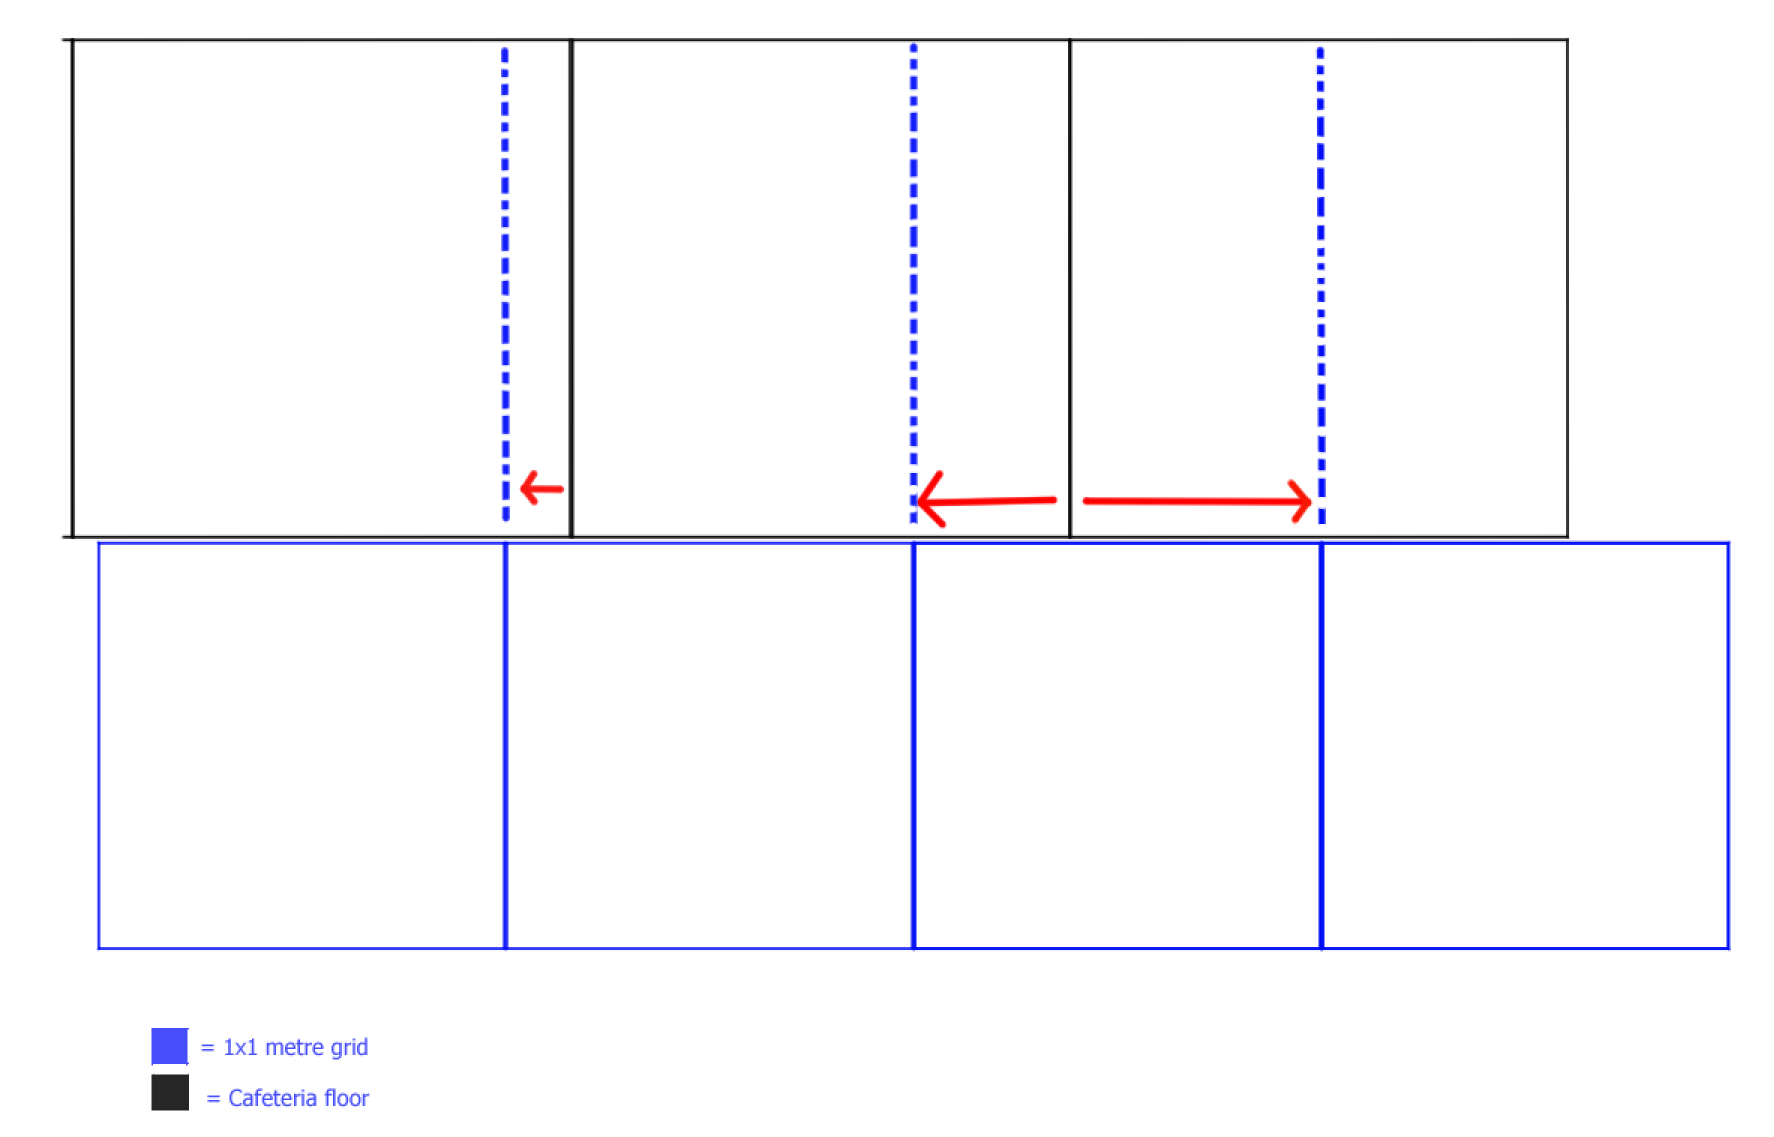
\includegraphics[width=\textwidth]{meth1.png}
	\caption{An overview of the research methodology. It divides the experiment into four main parts. (1) Identification of Environmental Factors, (2) Extraction of Environmental Factors, (3) Training of Fingerprint Matching Models, (4) Results and Evaluation}
	\label{fig:graph_step}
\end{figure}

\section{Research Methodology}
%\vspace{-15pt}
This paper adopts a systematic and empirical research methodology with the aim of identifying environmental factors that influence the IPS. This methodology is illustrated in Fig.~\ref{fig:graph_step}.

The figure illustrates the research methodology structured into four parts: (1) Identification of environmental factors, (2) Extraction of related data, (3) Training of fingerprint matching models, and~(4) Analysis and review of results. The research began by investigating environmental factors that potentially interfere with IPS performance through literature review and area analysis. Following data collection and analysis, fingerprint databases were generated. The investigation led to creating two datasets: one with different grid sizes and another with varying reference point numbers. These datasets trained various ML models including KNN, SVM, RF, MLP, XGBoost, and XGBoost-based RF (XBGRF), selected for their effectiveness in traditional classification tasks and accessibility. Grid size served as a key variable to determine and measure its impact on results and identify optimal configurations. Finally, the location prediction accuracy was analyzed and evaluated against ground truth data.

\subsection{Identification of Environmental Factors}
To begin collecting data for constructing the fingerprint database, the environment must first be mapped and prepared for data collection. An environmental map was created by taping the floor into grids matching the digital floor plan, as shown in Fig. \ref{fig:taping}. 

The tape serves as a reference point for the data collection device (a phone) when measuring RSSI values from nearby APs. The size and number of grids directly affects the collected datapoint quantity. Larger grid sizes reduce localization errors but decrease data point density. Different layouts and tiling across areas presented challenges, as certain floors had distinct tiling with varying elevations and angles. This was addressed by constructing grids based on previous reference points. 


An issue that presented itself was one concerning the different layout and tiling across different areas. Certain floors had distinct tiling with different elevation and angles. This was mitigated by constructing grids on previous reference points. Although minor measurement inaccuracies may exist, they are negligible for the purpose of this study.

While taping and collecting data points, another factor that could interfere with the IPS collection presented itself. The specific area inside the grid also affected how many RSSI values were present. For instance, collecting data in the top left corner of the grid could produce different RSSI values compared to the center of the grid. This issue could be addressed by either (1) removing the edge grids and (2) collecting fewer data points in the edge grid. However, both methods result in fewer data points being collected and have minimal impact on IPS performance. This is based on the assumption that, from a user experience perspective, being located at the edge of a grid represents a transitional state between adjacent grids. Meaning that, if misclassification occurs, it typically involves the neighboring grid and the correct grid itself. Therefore, for this study, the edge grid factor is negligible and omitted from further analysis.

\begin{figure}[!htbp]
	\centering
	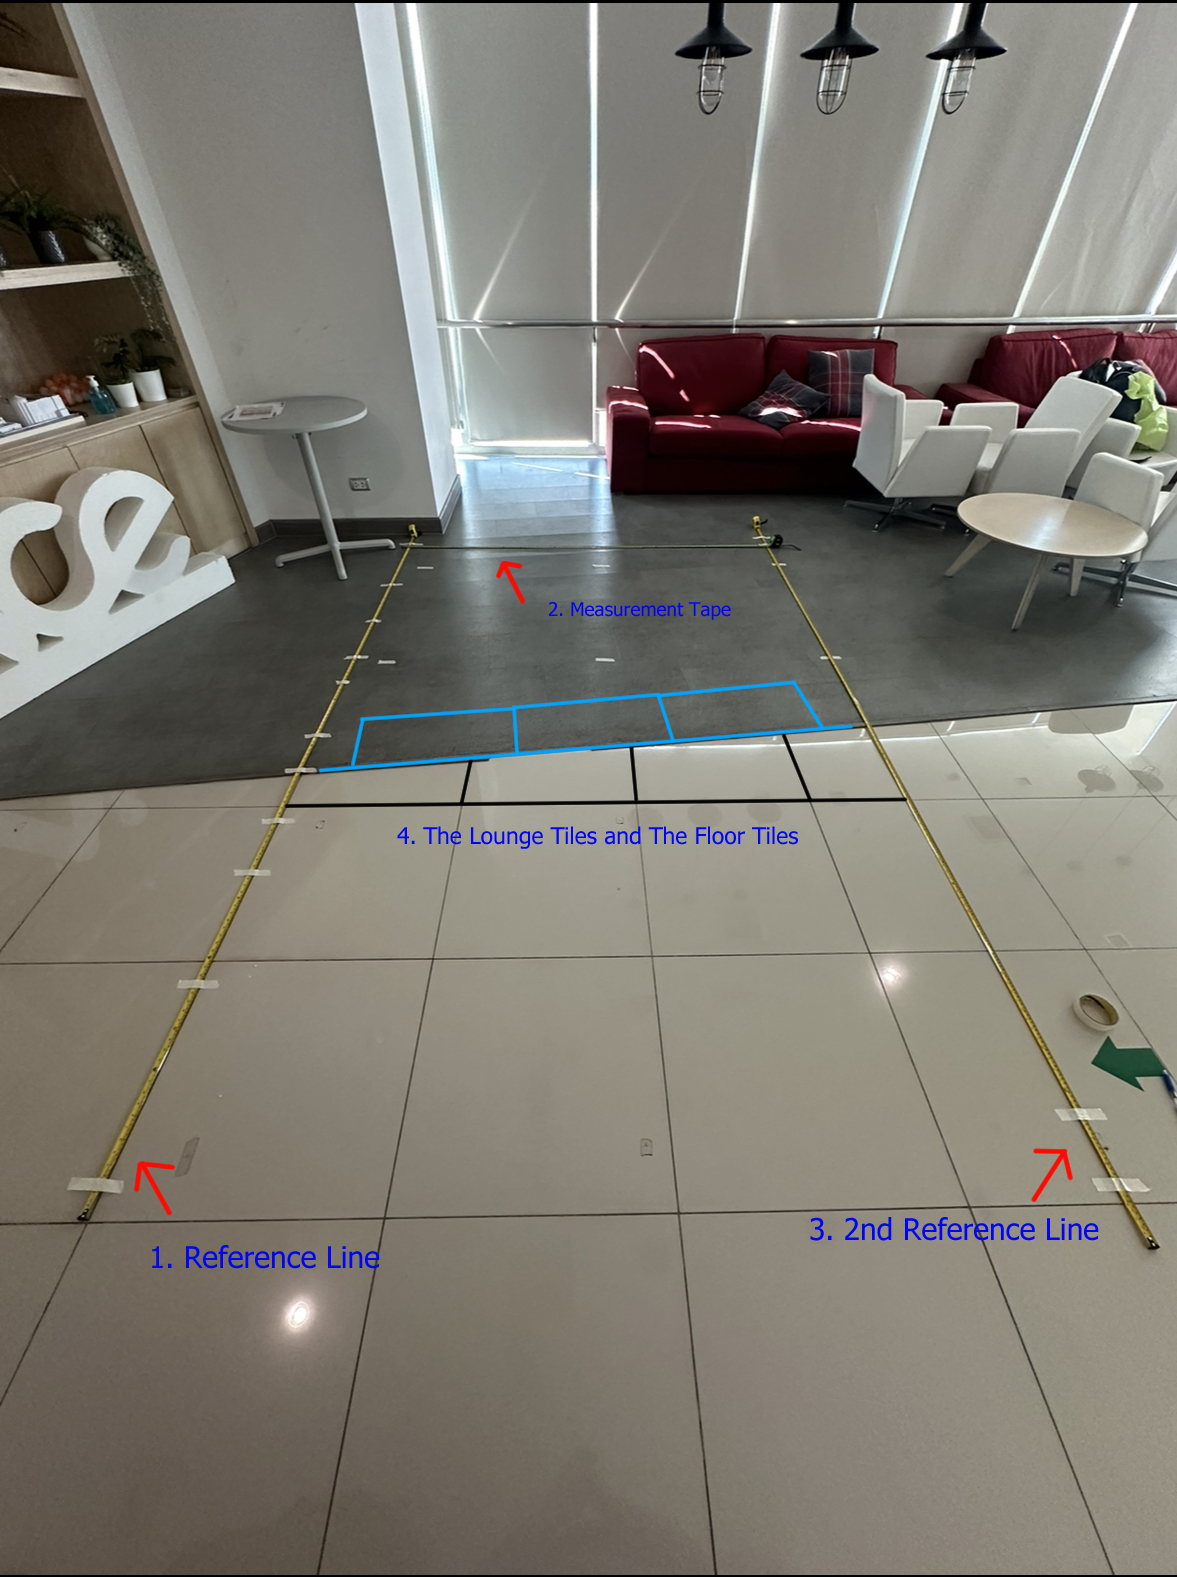
\includegraphics[width=\textwidth]{meth2.jpg}
	\caption{An example of taping that was done to create grids for data collection of RSSI values as fingerprints}
	\label{fig:taping}
\end{figure}

A similar issue arose concerning the alignment of the data structure used to assign unique labels to each grid across different floors. This challenge was particularly pronounced when experimenting with varying grid sizes, as the total area and layout of each floor differed significantly. Given the nature of this study, it was determined that the most practical approach was to treat each grid as a uniquely identifiable unit based on its grid ID. This decision was supported by the assumption that, in a classification model, sufficiently distinct features—such as differing numbers or distributions of BSSID signals observed in the same relative location on different floors—would enable the model to distinguish between grids effectively. Thus, treating each grid as uniquely distinct was not considered a limitation in this context.

To validate the assumption that each grid could be treated as a distinct unit across different floors, further analysis was conducted on the collected RSSI data. The data collection methodology initially captured all detectable access points within the network configuration, including those originating outside the intended environment. Access points from neighboring buildings were occasionally included in the dataset. Although these external access points typically exhibit low signal strength, their presence could influence the training of fingerprint-based localization models, introducing effects similar to zero-inflated spatial data.

To mitigate this issue and prevent feature space complexity, a filtering criterion was applied that retained only access points associated with the specific campus network. This ensured the dataset focused on relevant features while maintaining consistency across grids.
As illustrated in the heatmap in Fig. \ref{fig:heatmap008} (included here for supplementary context), some access points still exhibit non-zero RSSI values despite being on the lower end of the signal strength spectrum. These low-strength signals, represented by the darker regions on the map, may pose challenges for machine learning models during training by introducing noise and increasing the risk of underfitting.
Through this analysis, two key factors emerged as most influential in determining IPS performance: grid size, involving a trade-off between localization precision and data collection practicality, and the presence of low-relevance RSSI values that could adversely impact model performance if unfiltered. These findings support treating each grid as a unique unit, as both physical and feature-based variations across floors reinforce their distinctiveness.

\begin{figure}[htbp]
	\centerline{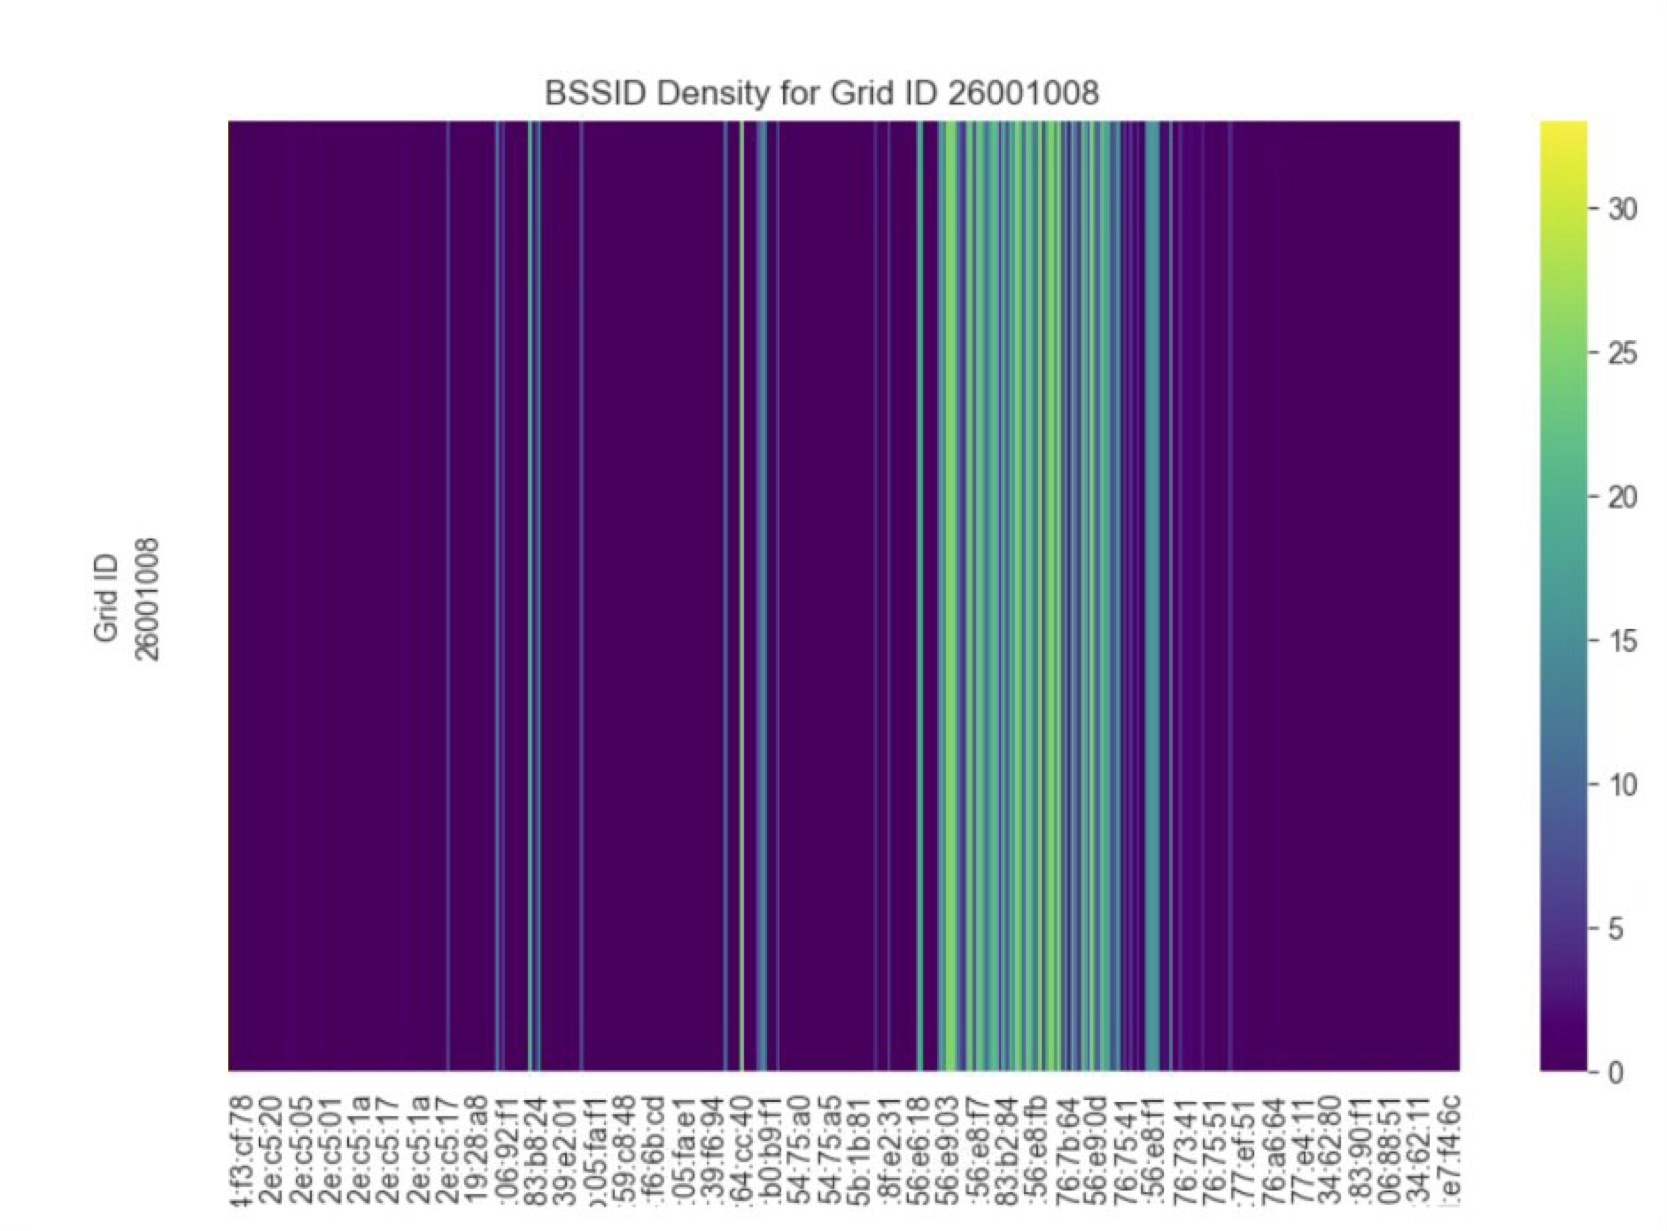
\includegraphics[scale=0.15]{meth3.jpg}}
	\caption{A heatmap that shows different access point’s RSSI values (referred to as BSSID) for a grid.}
	\label{fig:heatmap008}
\end{figure}

\subsection{Extraction of Environmental Factors and Datasets}
The identification of the two factors in the previous section enables adjustments to find optimal settings for maximizing IPS performance. 
To support this evaluation, two key metrics are defined for this study: Average Grid from Target (AGT) and Average Distance from Target (ADT).

\begin{equation}
	AGT = \sqrt{(\Delta X)^2 + (\Delta Y)^2}
	\label{eq:agt}
\end{equation}
$\Delta X$ and $\Delta Y$ represent horizontal and vertical axes, respectively. This formulation stems from treating each grid as a discrete unit within the map. Given that the grid layout inherently defines the number of divisions along the $X$ and $Y$ axes, offset can be directly computed as the distance between predicted and actual grid positions. Treating offsets as distance units, the measure naturally adapts to different grid sizes, providing a straightforward means to visualize performance and a standardized measure across different grid sizes.

\begin{equation}
	ADT = AGT \times \sqrt{{g_w}^2 + {g_h}^2}
	\label{eq:adt}
\end{equation}
$g_w$ and $g_h$ denote the grid width and height, respectively. While AGT captures classification error in grid labels, ADT introduces a precision-accuracy trade-off by scaling AGT with the grid’s diagonal distance. Low AGT may correspond to poor precision if grid sizes are large. The use of the full diagonal length introduces a penalty to grid merging: rather than calculating precise physical distances, ADT provides a practical and realistic means of visualizing the precision-accuracy trade-off while not being constrained by traditional GPS accuracy, which suffers indoors.

\paragraph{Grid Size Requirements and Datasets} Grid size influences IPS performance. Its size influences the accuracy of the algorithm, as well as the ease of data collection. The following study \cite{LRE1} ran a model with grid sizes of 16.75 x 15m and reported high IPS performance in terms of AGT, as the larger the area, the more likely you’ll estimate the correct grid. The trade off was that the ADT was significantly lower, as there was a deviation from the actual point. This suggests that by minimising the grid size, we can achieve a higher precision. However the lower the precision, the harder the data collection process. 
Collecting data for varying grid sizes via the taping method is impractical, as repeatedly taping the area is not feasible for a small team. To address this, RSSI value interpolation was employed to generate larger grid sizes by aggregating smaller grids. The data collected from small grids (1m x 1m) is aggregated to construct larger grids by interpolating RSSI values from the combined smaller grids.

By collecting 5 datapoints in a grid (top left, top right, bottom left, bottom right and centre), these RSSI values can be interpolated into a combined grid by averaging the values from the individual grids.

For example, when creating a 2m x 2m grid, this is done by determining a value where the sum of distances between the RSSI values of the centres are all 0 in all four grids and then interpolating them. This method works as the grid sizes were 1m x 1m grids. The reliability of these interpolated grids is consistent, as they use the same dataset with different conceptual grid sizes.

\begin{figure}[htbp]
	\centerline{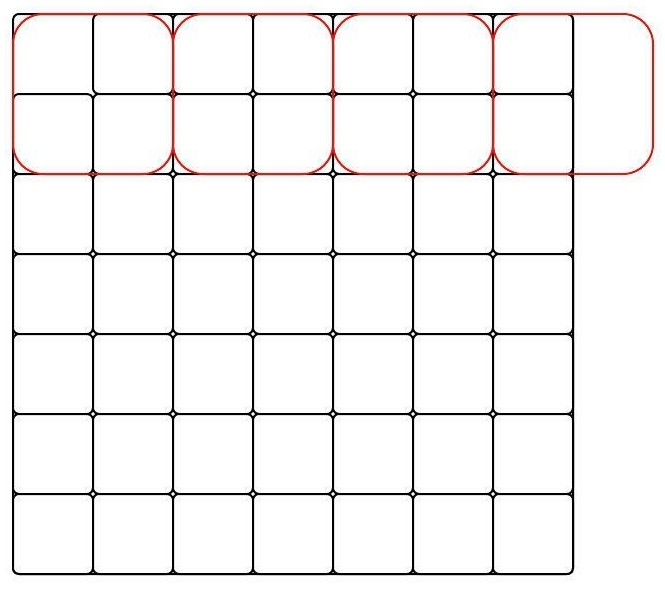
\includegraphics[scale=0.5]{image14.jpg}}
	\caption{Visualizing grid resizing}
	\label{fig:vis_grid_resize}
\end{figure}

\paragraph{Unrelated RSSI Value Filtering and Datasets} Many points exhibit low RSSI values as shown previously in fig. \ref{fig:heatmap008}. To avoid underfitting, these values were omitted from the model. However, the removal of these values does not guarantee improved accuracy. To measure this, two datasets were created: one with all access points and one with omitted RSSI values. Comparing the results of both datasets determines the impact of these omitted values on IPS performance.

White-listing of access points within the targeted area was also considered, but this was deemed unnecessary as it would result in the dataset exhibiting characteristics similar to an unfiltered dataset for a multi-floor model.


\section{Result}
\begin{table}[htbp]
	\centering
	\begin{minipage}{0.42\textwidth}
		\centering
		\caption{Total True Unique Grids by Floor}
		\label{tab:true_unique_grid}
		\vspace{2pt}
		\small
		\begin{tabular}{|l|c|c|} 
			\hline
			& \multicolumn{2}{c|}{\textbf{Floor}}  \\ 
			\hline
			\textbf{1x1 Grid Size} & 1st & 2nd \\ 
			\hline
			\textbf{Grid Count} & 309 & 174 \\
			\hline
		\end{tabular}
	\end{minipage}
	\hfill
	\begin{minipage}{0.52\textwidth}
		\centering
		\caption{Total BSSID Before and After Filtering}
		\label{tab:bssid_counts}
		\vspace{2pt}
		\small
		\begin{tabular}{|l|l|c|}
			\hline
			\multicolumn{2}{|l|}{\textbf{Collected Data Points}} & \textbf{\# BSSID} \\
			\hline
			\multirow{2}{*}{\textbf{Filtering}} & Non-Filtered & 1799 \\
			\cline{2-3}
			& Filtered & 378 \\
			\hline
		\end{tabular}
	\end{minipage}
\end{table}
\vspace{-15pt}
\begin{table}[htbp]
	\caption{Total Unique Grids for Each Grid Size Experiment}
	\label{tab:grid_size_variations}
	\vspace{2pt}
	\centering
	\small
	\begin{tabular}{|l|c|c|c|c|c|c|c|c|} 
		\hline
		\textbf{Grid Size} & 1x1 & 3x3 & 5x5 & 7x7 & 9x9 & 11x11 & 13x13 & 15x15 \\ 
		\hline
		\textbf{Total Grids} & 483 & 96 & 47 & 29 & 28 & 16 & 18 & 9 \\
		\hline
	\end{tabular}
\end{table}
\vspace{-10pt}

The dataset used in this study consisted of 12,640 data points collected across 1x1m\textsuperscript{2} grids distributed among the floors of the experimental setup. Filtering the available BSSID to utilize only SSID with specific identifiers resulted in 378 unique BSSID spanning across the 2 floors. The rationale behind filtering WiFi signals is to determine whether only easily identifiable BSSID can be utilized in implementing IPS. 9019 data points were collected on the 6th floor and 3621 data points on the 7th floor.

To explore how different parameter settings impact model training, various configurations were systematically tested, training the model multiple times under each setting. The table below highlights the best results observed. Notably, the highest accuracy and the best AGT do not come from the same parameter setting.

%\begin{equation}
%	AGT = \sqrt{(offset\_X)^2 + (offset\_Y)^2} 
%\end{equation}


This suggests that these metrics prioritize different aspects of performance—optimizing for accuracy does not necessarily yield the best AGT and vice versa. This insight provides a key perspective for analyzing the results in detail. Additionally, according to fig. ~\ref{fig:AGT_dgrid_size}, from 7x7m grid size onwards, the best AGT measured across different models starts to plateau, indicating diminishing returns from increasing experiment grid size.

\begin{comment}
	\begin{figure}
		\centering
		\begin{subfigure}{0.4\textheight}
			\centerline{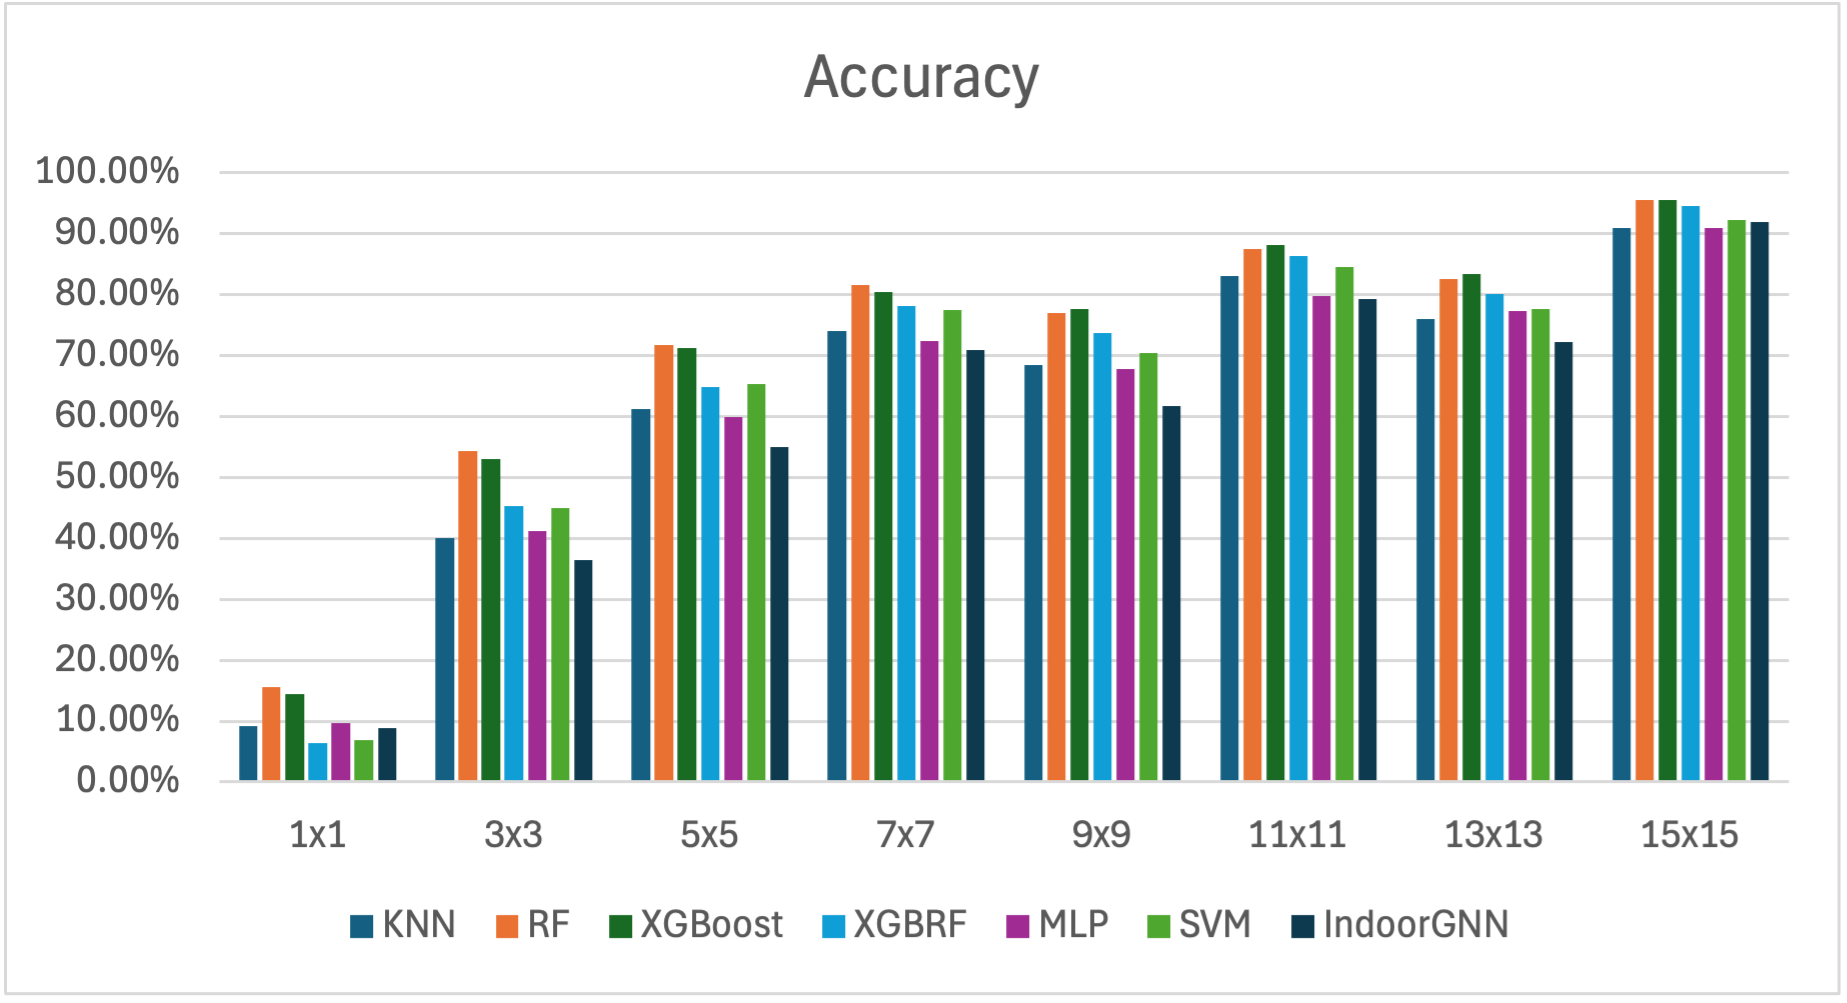
\includegraphics[scale=0.65]{image3.png}}
			\caption{Model Accuracy on Different grid size}
			\label{fig:acc_dgird_size}
		\end{subfigure}
		\hfill
		\begin{subfigure}{0.4\textheight}
			\centerline{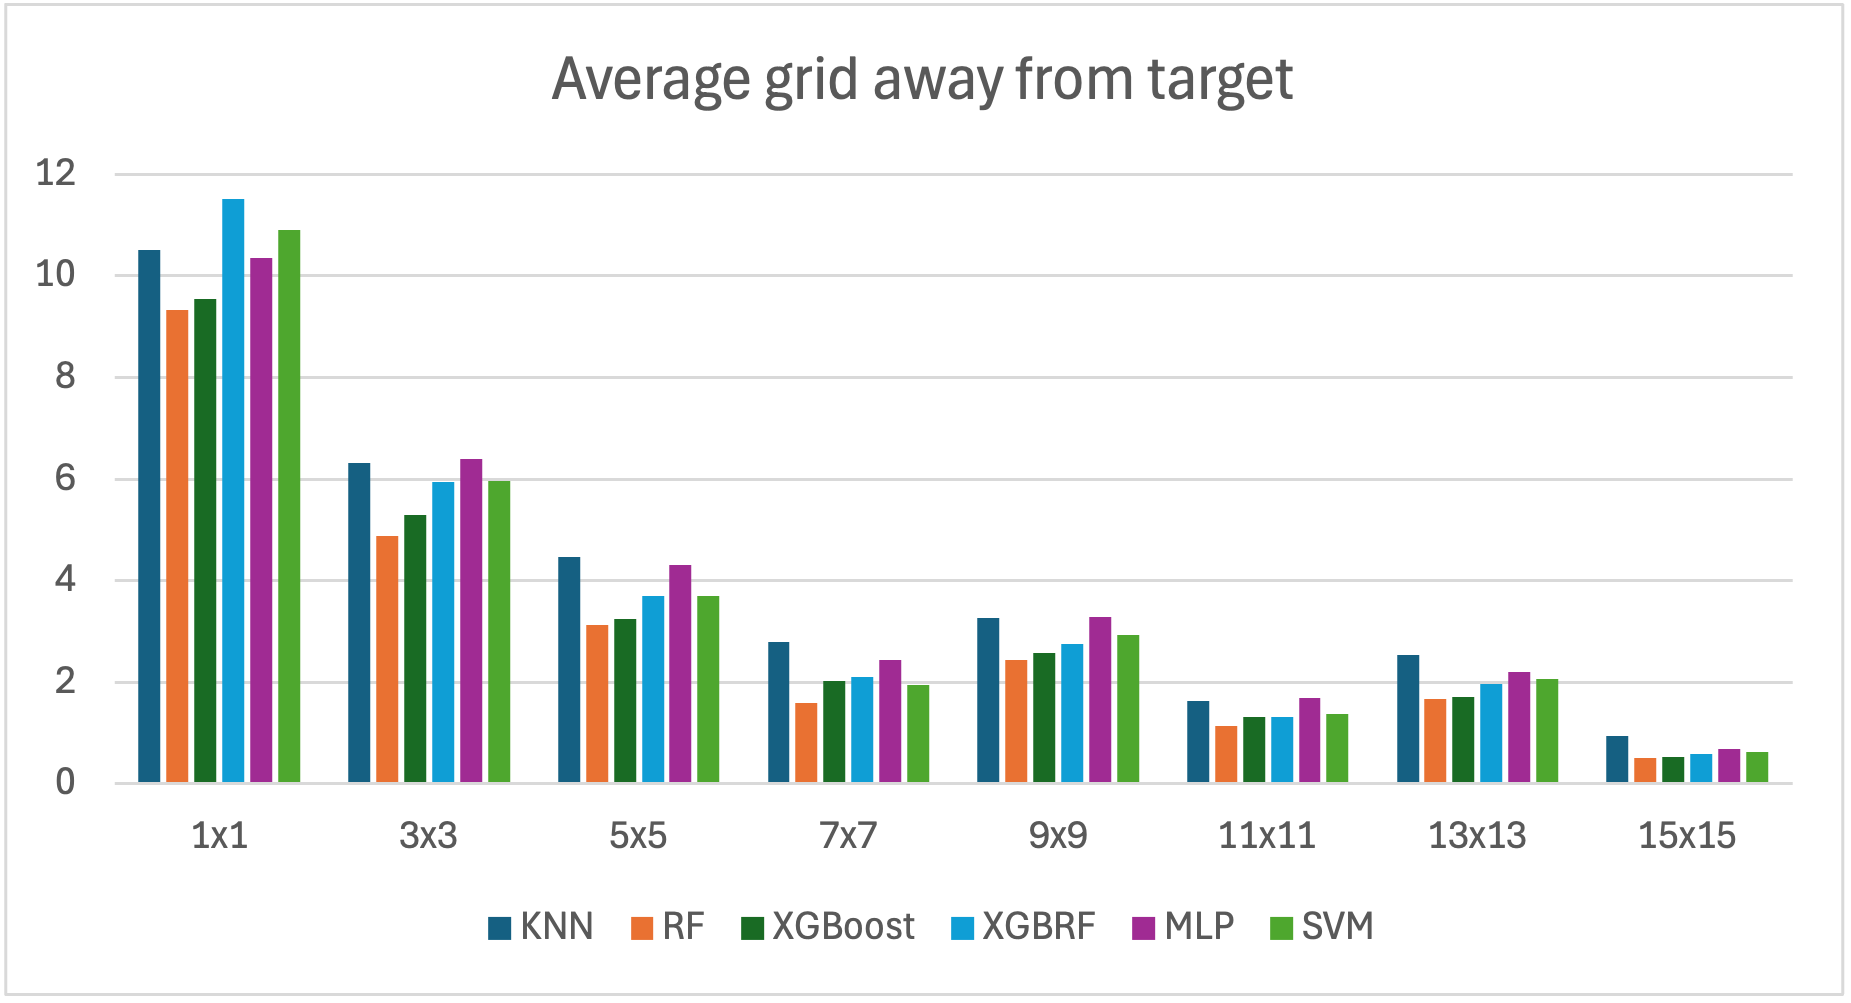
\includegraphics[scale=0.65]{image1.png}}
			\caption{Model Average grid away from Target on Different grid size}
			\label{fig:AGT_dgrid_size}
		\end{subfigure}
	\end{figure}
\end{comment}

\begin{comment}
	\begin{figure}[htbp]
		\centering
		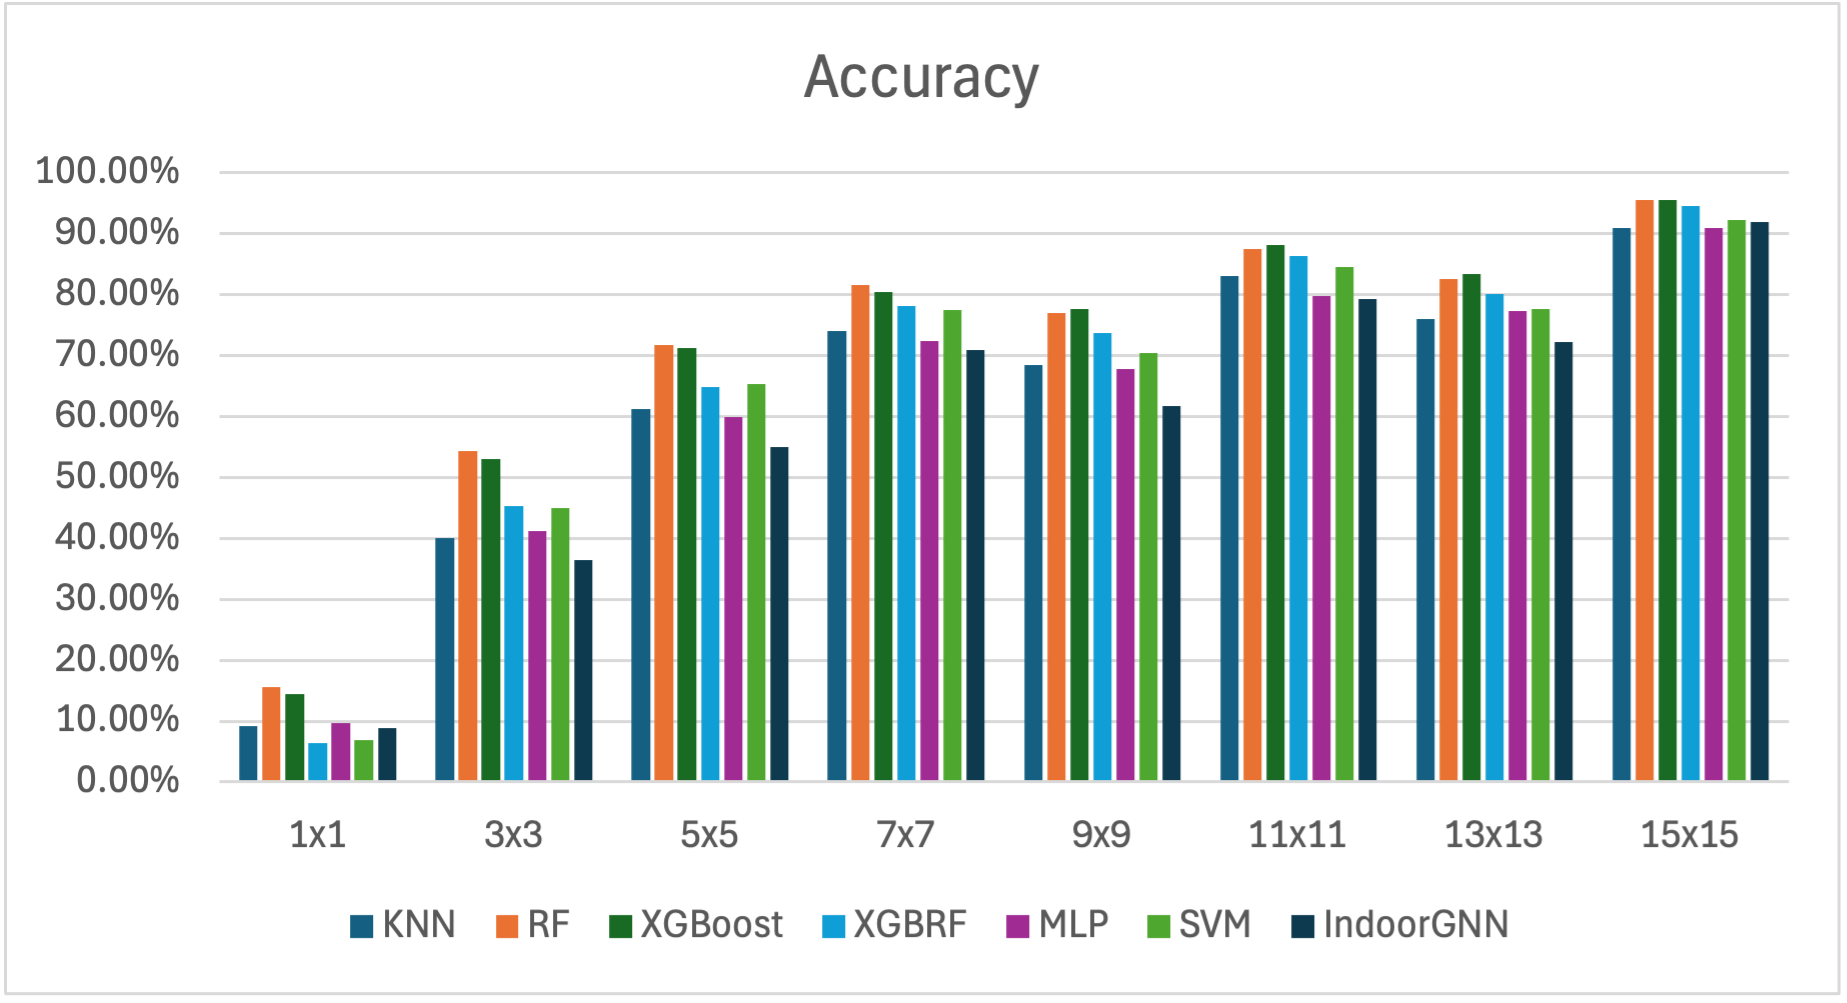
\includegraphics[scale=0.8]{image3.png}
		\caption{Model Accuracy on Different grid size}
		\label{fig:acc_dgird_size}
	\end{figure}
	
	\begin{figure}[htbp]
		\centering
		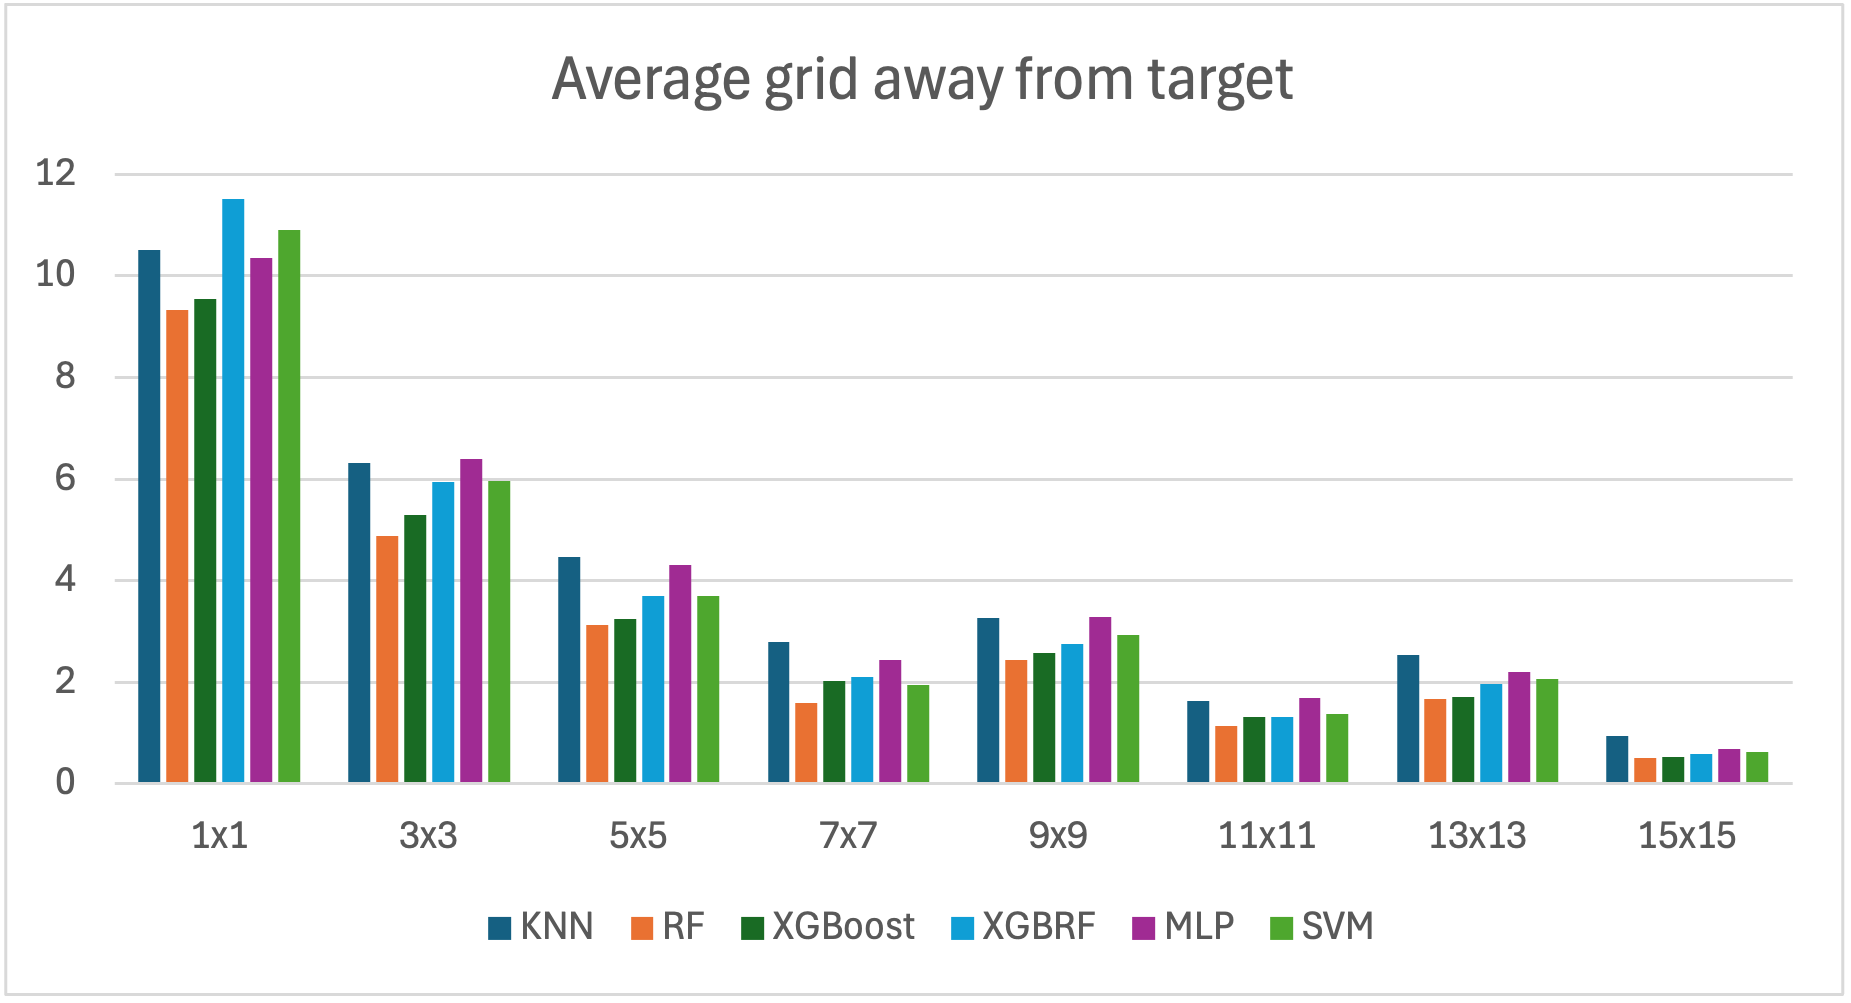
\includegraphics[scale=0.65]{image1.png}
		\caption{Model Average grid away from Target on Different grid size}
		\label{fig:AGT_dgrid_size}
	\end{figure}
\end{comment}

\vspace{-10pt}
\begin{figure}[hbt!]
	\begin{minipage}{0.45\textwidth}
		\centering
		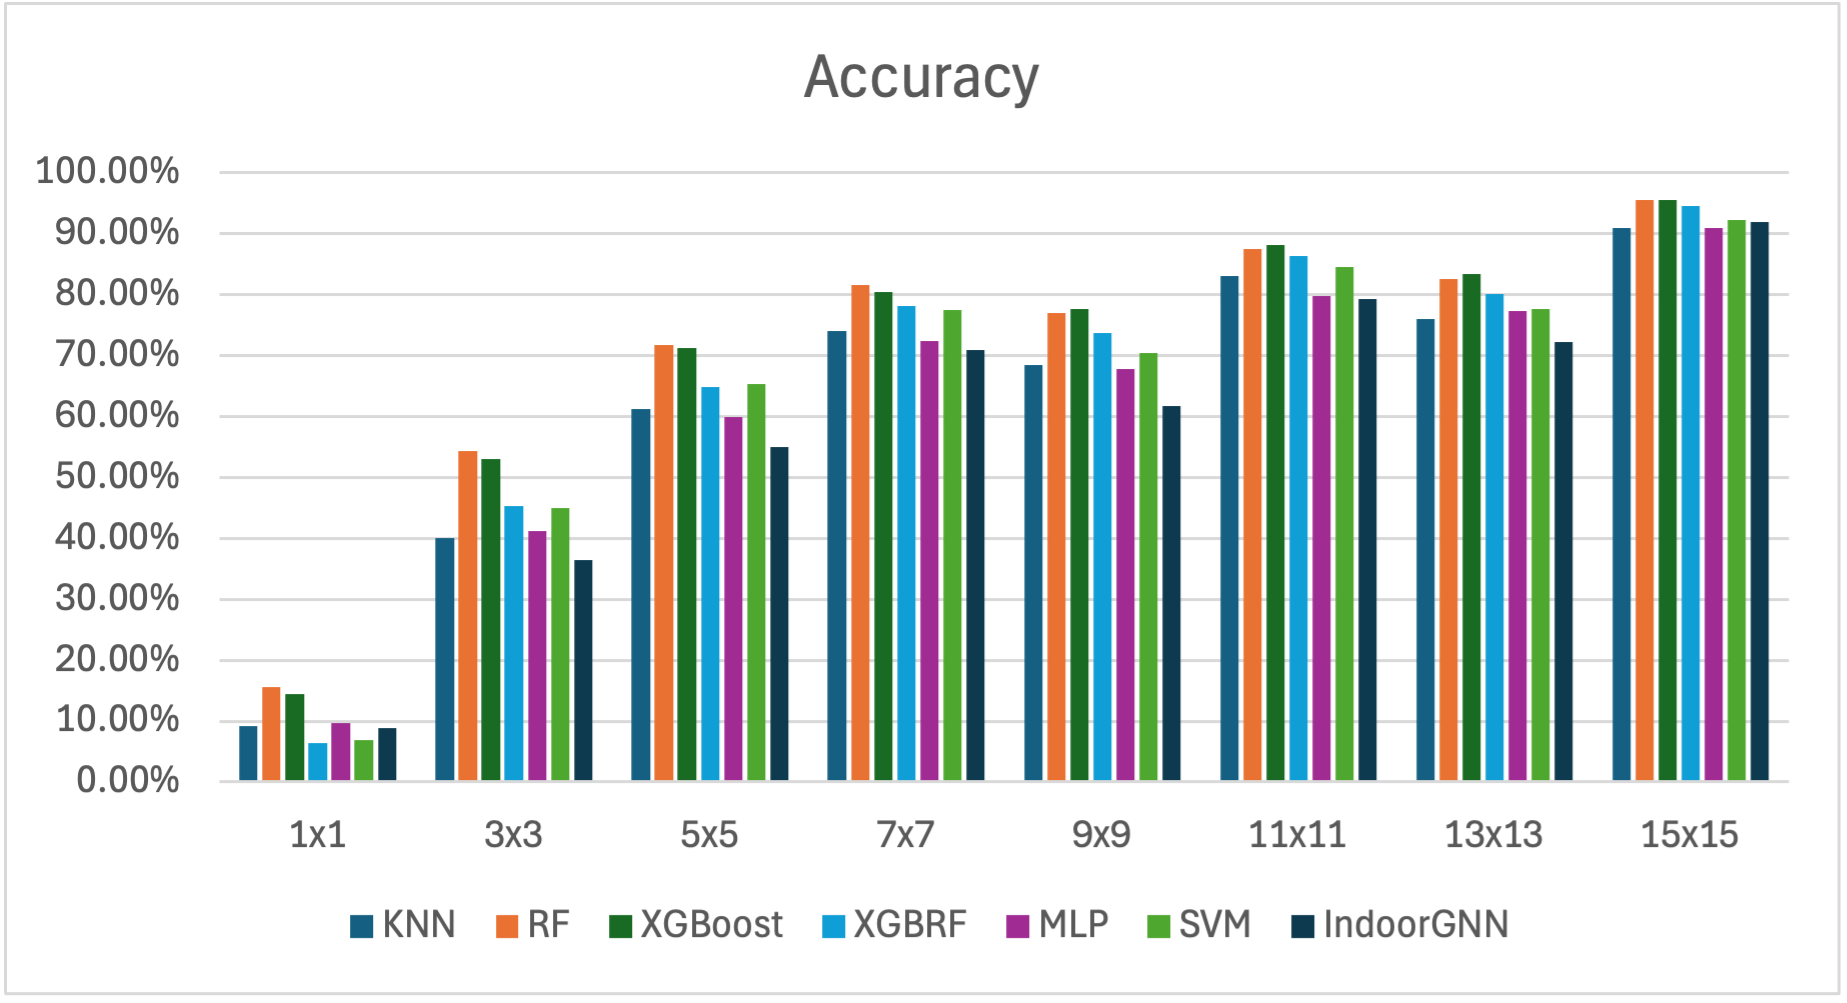
\includegraphics[scale=0.5]{image3.png}
		\caption{Model Accuracy on Different grid size}
		\label{fig:acc_dgird_size}
	\end{minipage}
	\hfill
	\begin{minipage}{0.45\textwidth}
		\centering
		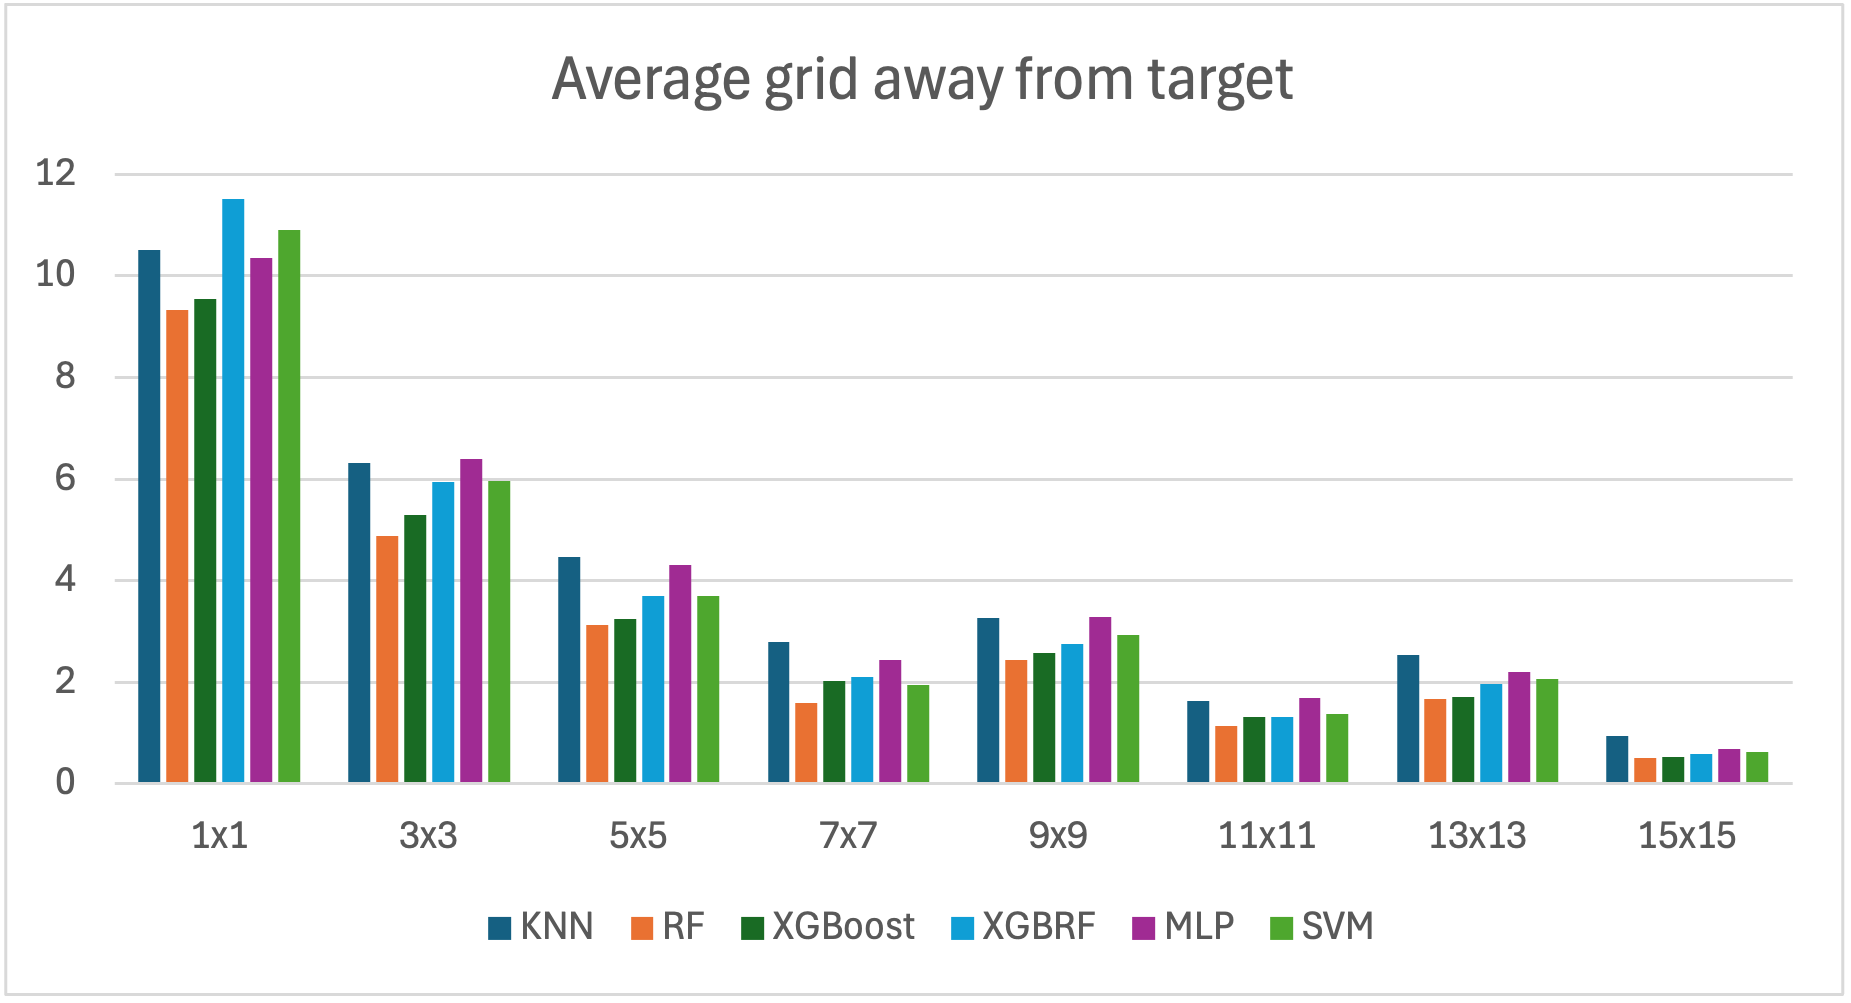
\includegraphics[scale=0.5]{image1.png}
		\caption{Model Average grid away from Target on Different grid size}
		\label{fig:AGT_dgrid_size}
	\end{minipage}
\end{figure}

\vspace{-30pt}
\section{Discussion}
%\vspace{-10pt}
By conducting experiments across multiple grid sizes, the tradeoff between grid size and precision can be visualized. To quantify this, the average grid deviation from the target is calculated and multiplied by each grid size's diagonal length, as shown in fig. \ref{fig:AGT_dgrid_size}. This illustrates the expected deviation in predictions when a model is trained on a specific grid size, should an error occur.

While a 15x15m grid size performs well on the graph, it inherently limits accuracy to that resolution. In cases where predictions are correct, the location remains constrained within a 15×15m area, which may not be suitable for applications requiring higher precision—such as those needing to pinpoint areas smaller than this grid size.

Through this experiment, a 7x7m grid size was found to offer the best balance between accuracy and precision. The ADT demonstrates that utilizing a 7x7m grid size minimizes error while remaining small enough for precision-dependent applications. 

However, these findings may not generalize to all IPS implementations in different environments. The results suggest that increasing grid size does not necessarily improve accuracy or precision; in some cases, performance actually declines, as shown in the chart. This highlights the need for careful consideration when selecting a grid size based on specific IPS deployment requirements.


%\begin{equation}
%	ADT = AGT \times \sqrt{(grid\_width)^2 + (grid\_height)^2}.
%\end{equation}

\begin{figure}[htbp]
	\centerline{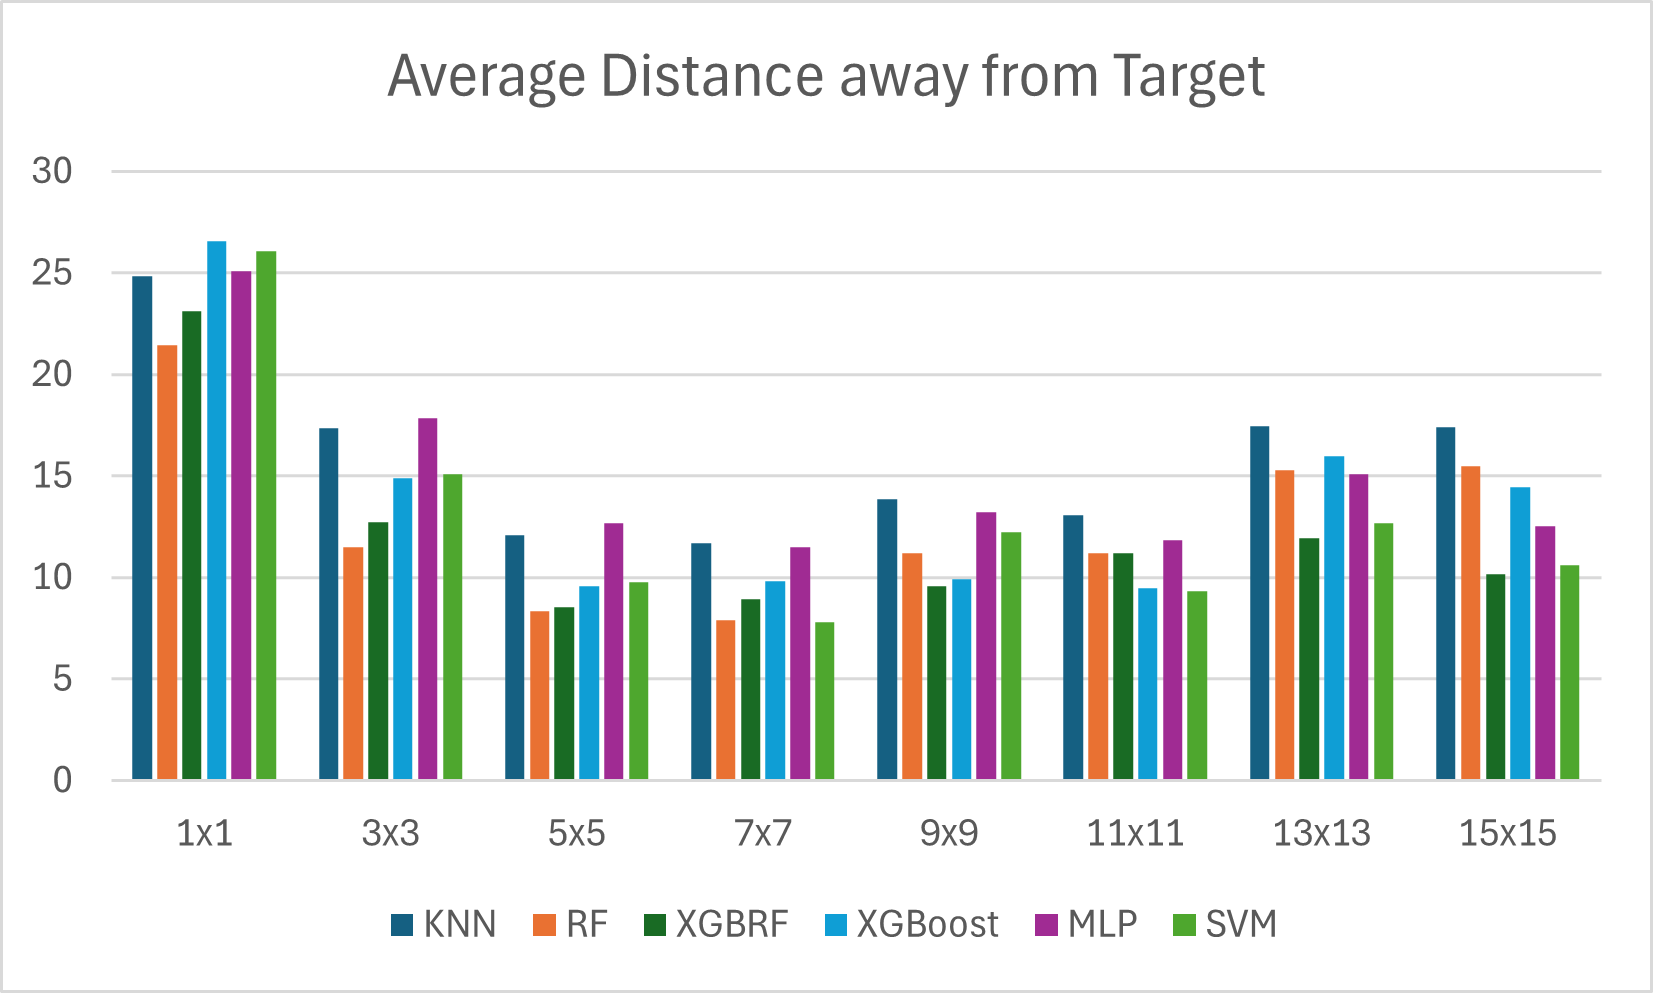
\includegraphics[scale=0.65]{image2.png}}
	\caption{Average Distance Error Across Different Grid Resolutions}
	\label{fig:Avg_dis_err}
\end{figure}

Training an IPS model involves significant computational challenges, particularly when dealing with high-dimensional feature spaces. The experiment implemented a simple Wi-Fi access point filtering approach, selecting only access points containing specific identifiers in their names. This drastically reduced the number of access points used as features, making the training process more efficient.

\begin{figure}[hbt!]
	\centering
	% First row
	\begin{minipage}{0.45\textwidth}
		\centering
		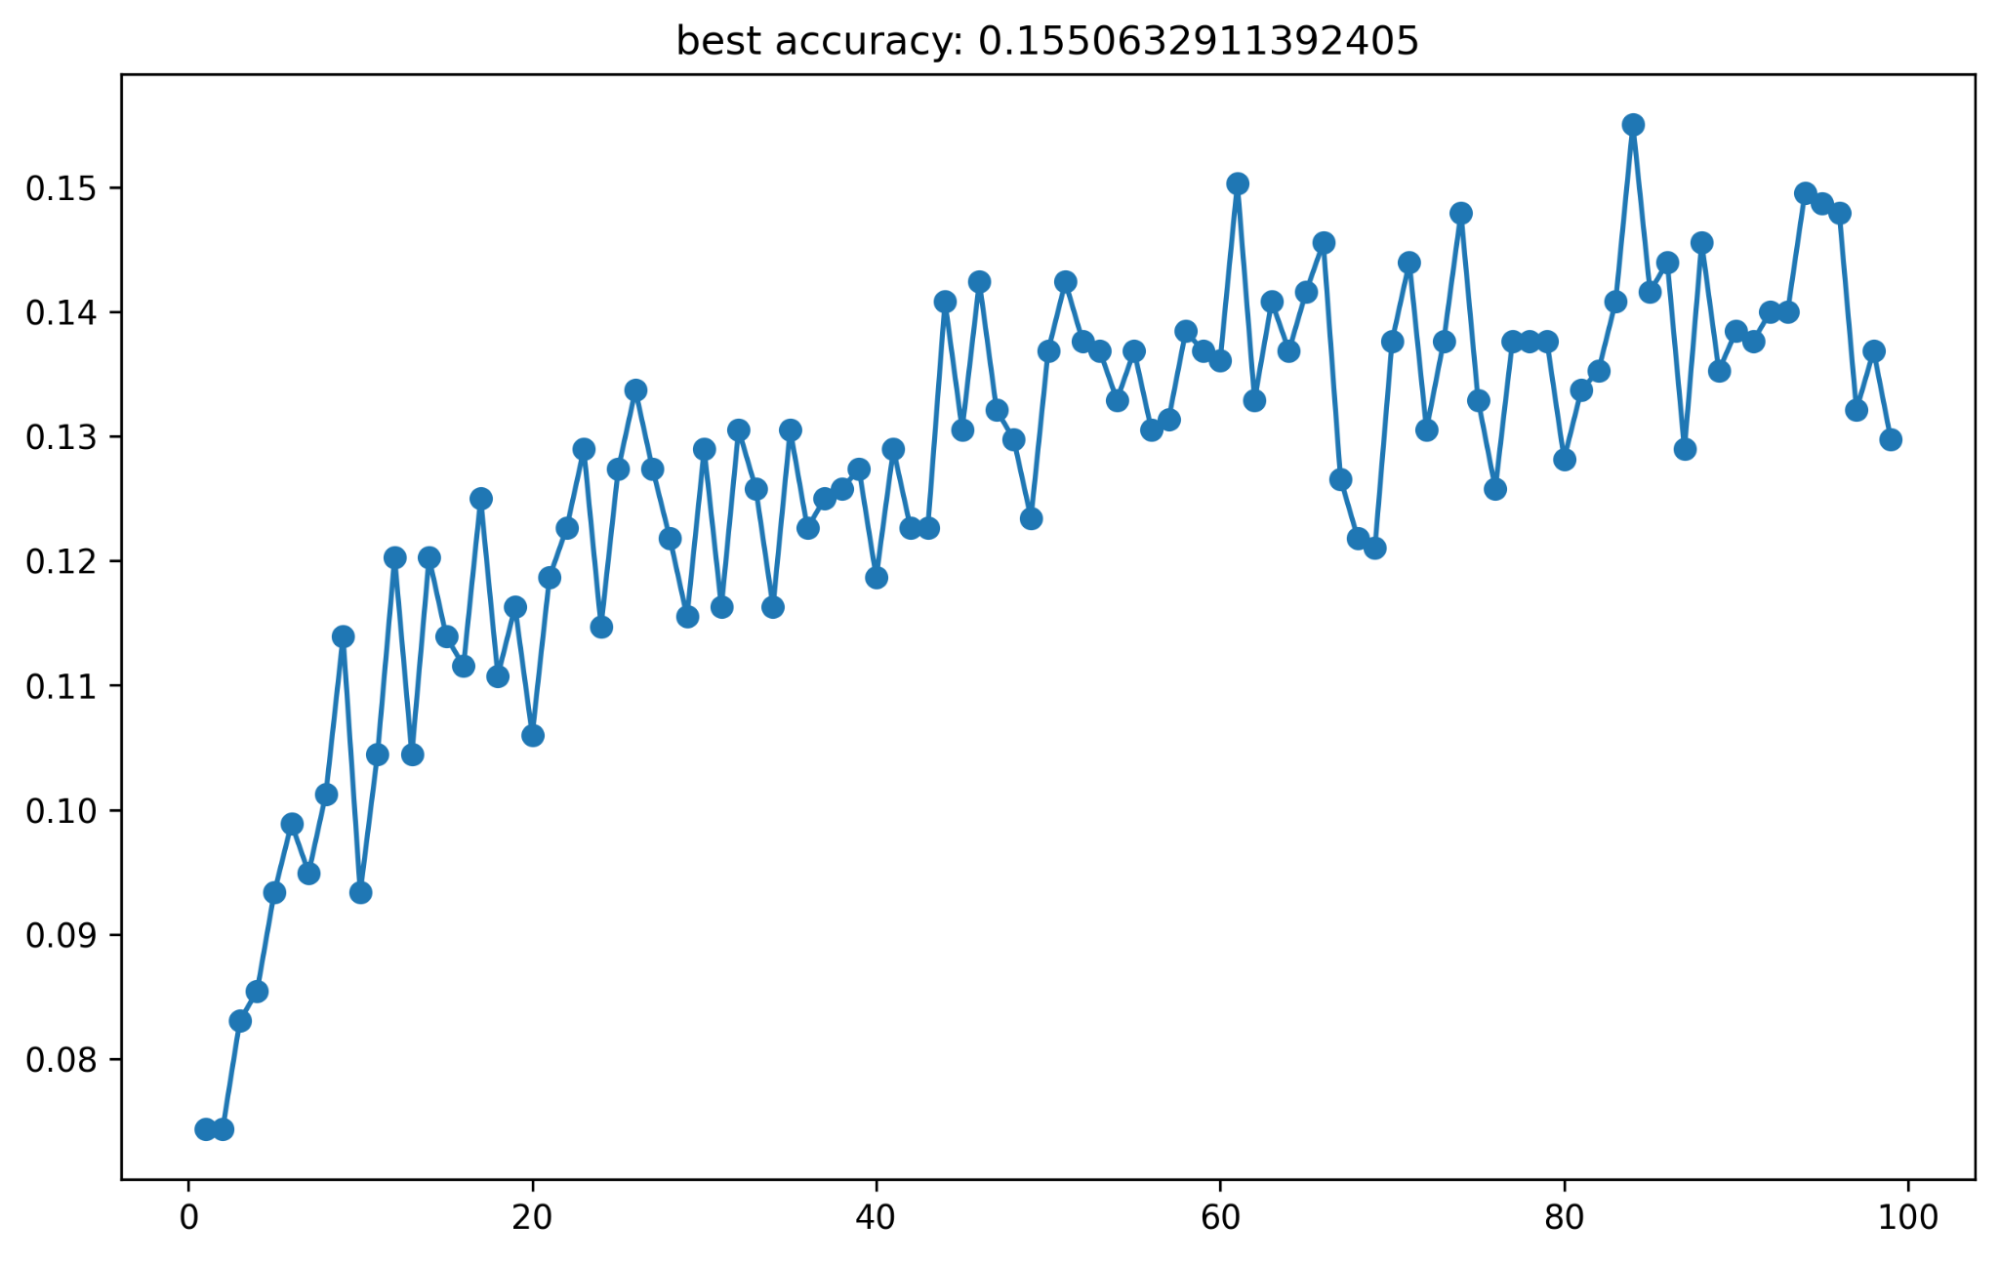
\includegraphics[width=\linewidth]{image5.png}
		\caption{RF Model accuracy with BSSID filtering (1x1)}
		\label{fig:rf_acc_filter}
	\end{minipage}
	\hfill
	\begin{minipage}{0.45\textwidth}
		\centering
		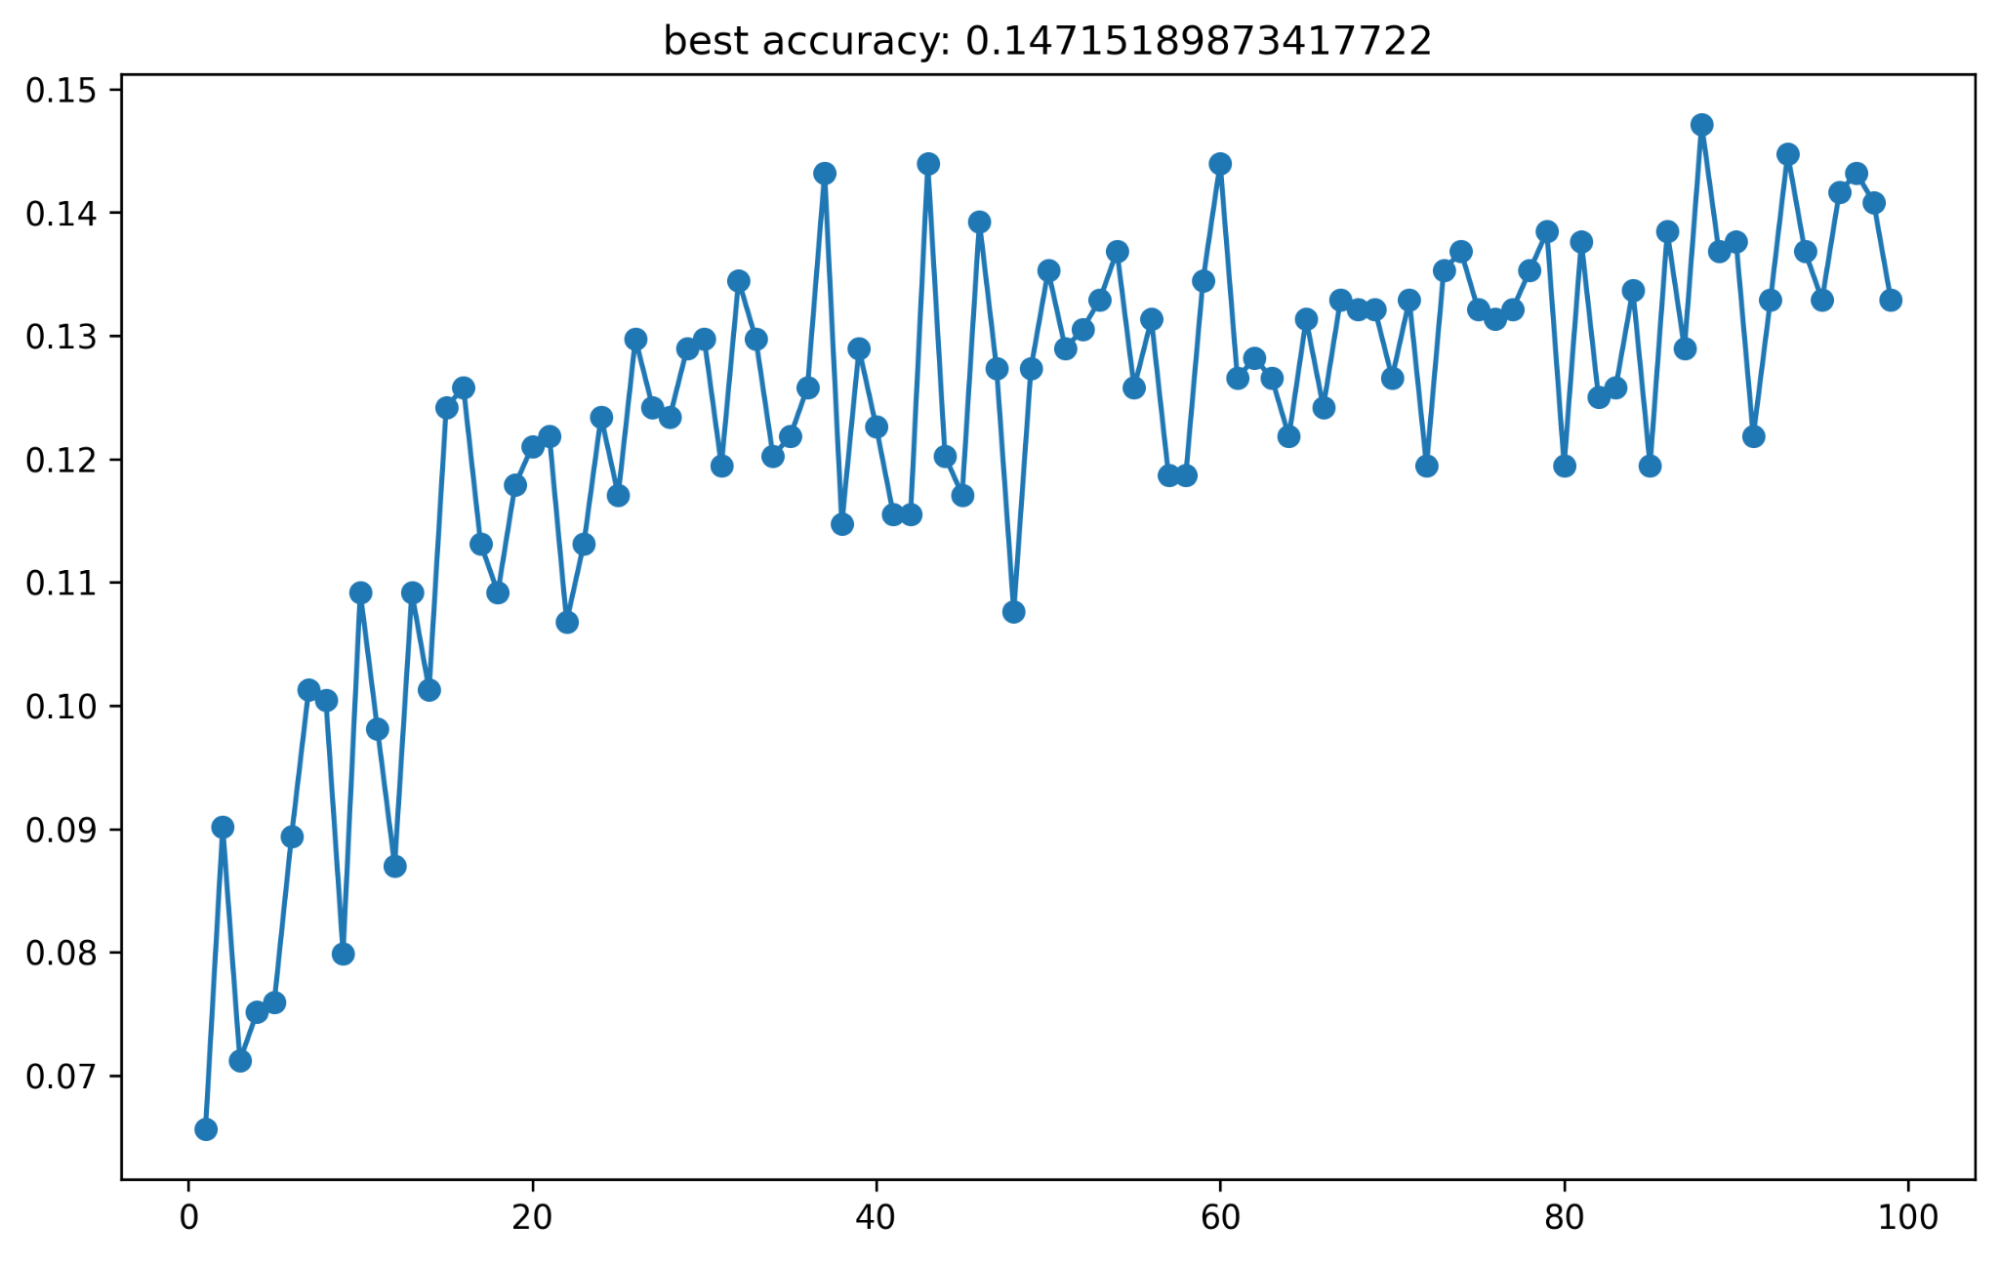
\includegraphics[width=\linewidth]{image6.png}
		\caption{RF Model accuracy without BSSID filtering (1x1)}
		\label{fig:rf_acc_nofilter}
	\end{minipage}
	
	\vspace{0.5cm} % vertical space between rows
	
	% Second row
	\begin{minipage}{0.45\textwidth}
		\centering
		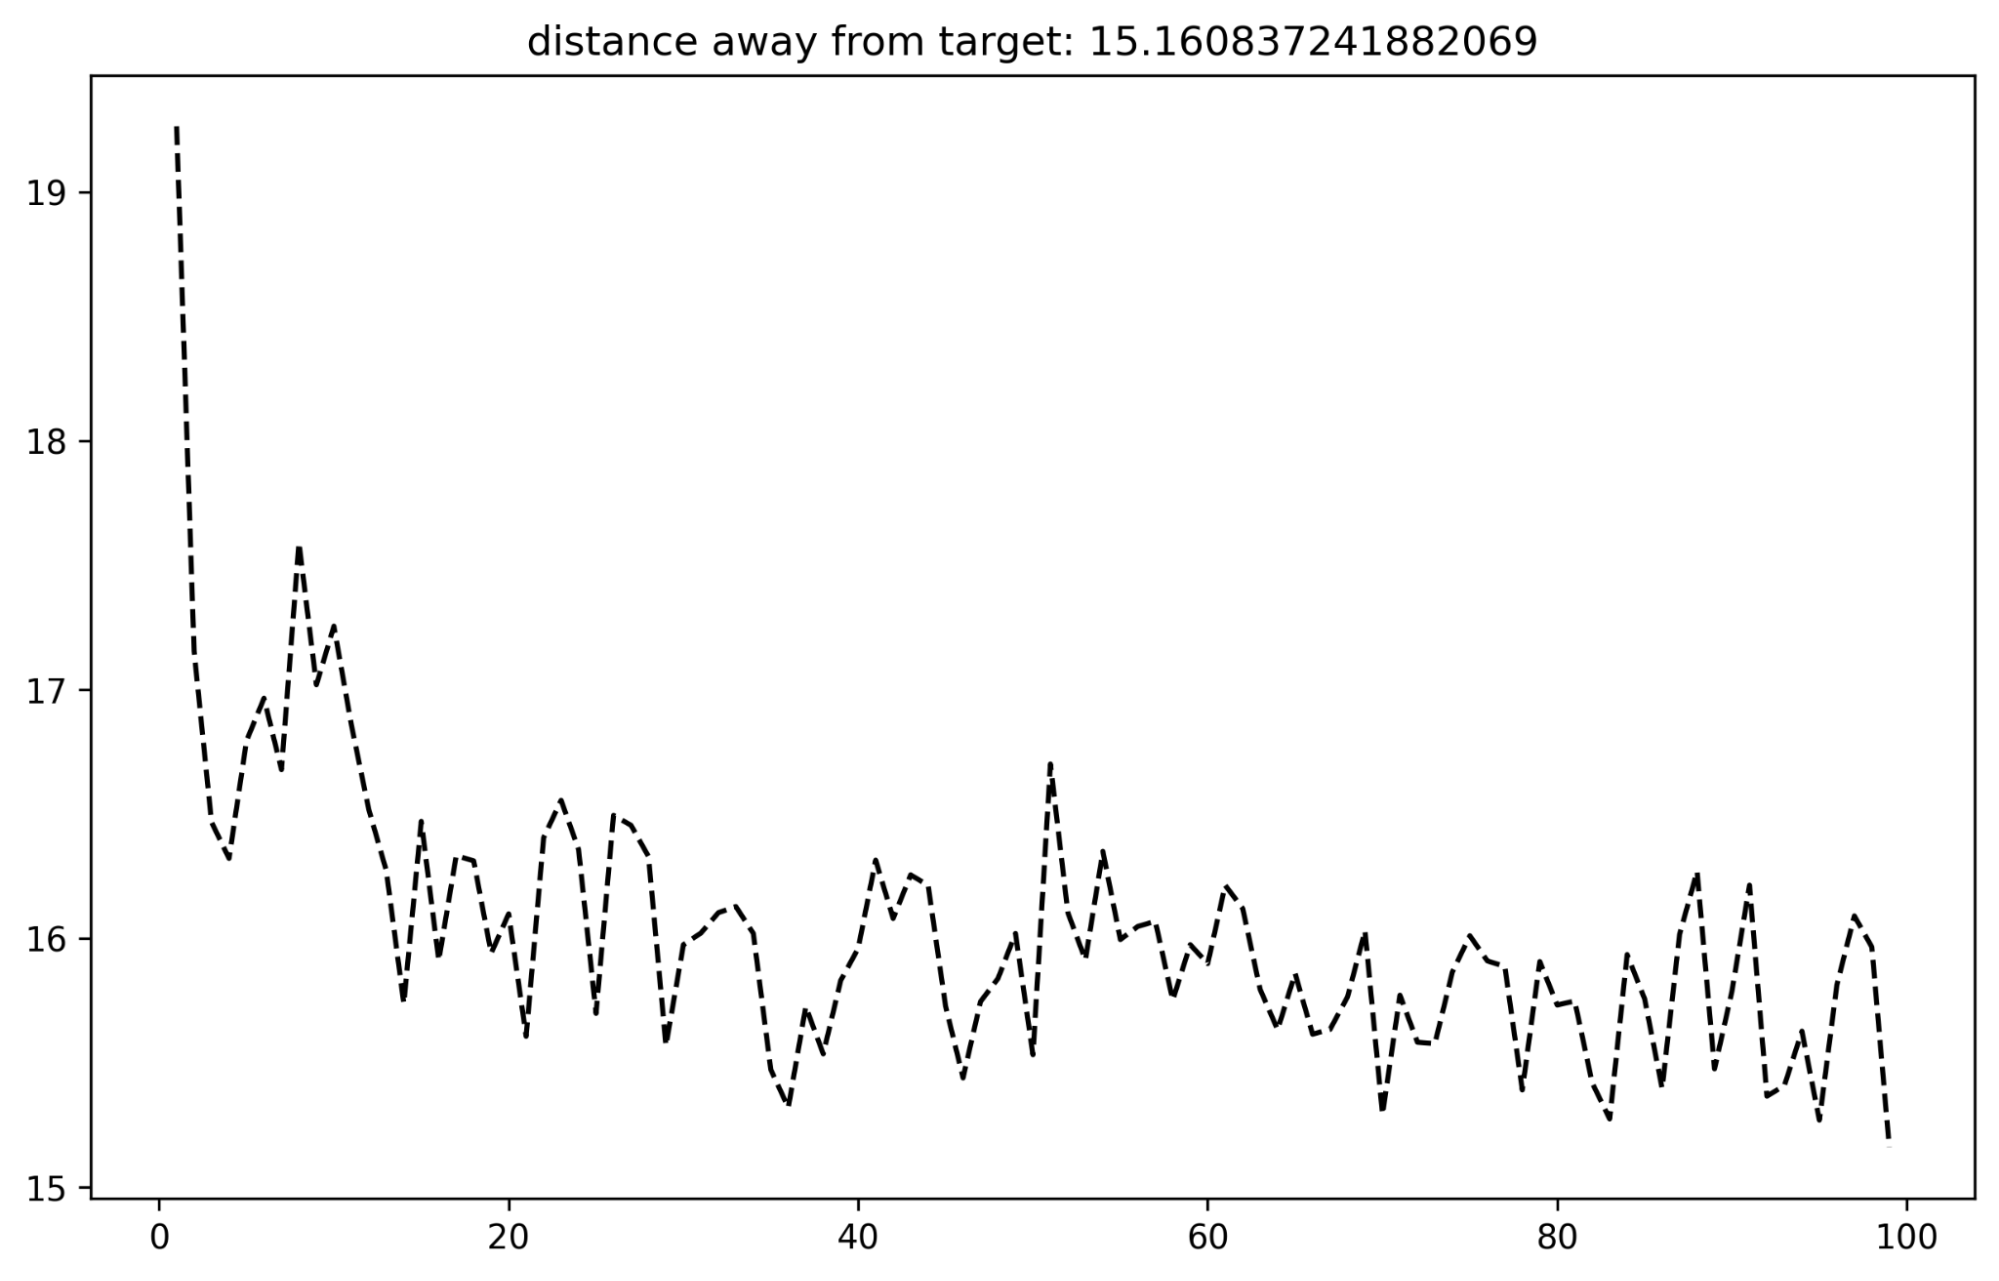
\includegraphics[width=\linewidth]{image4.png}
		\caption{RF Model AGT with BSSID filtering (1x1)}
		\label{fig:rf_agt_filter}
	\end{minipage}
	\hfill
	\begin{minipage}{0.45\textwidth}
		\centering
		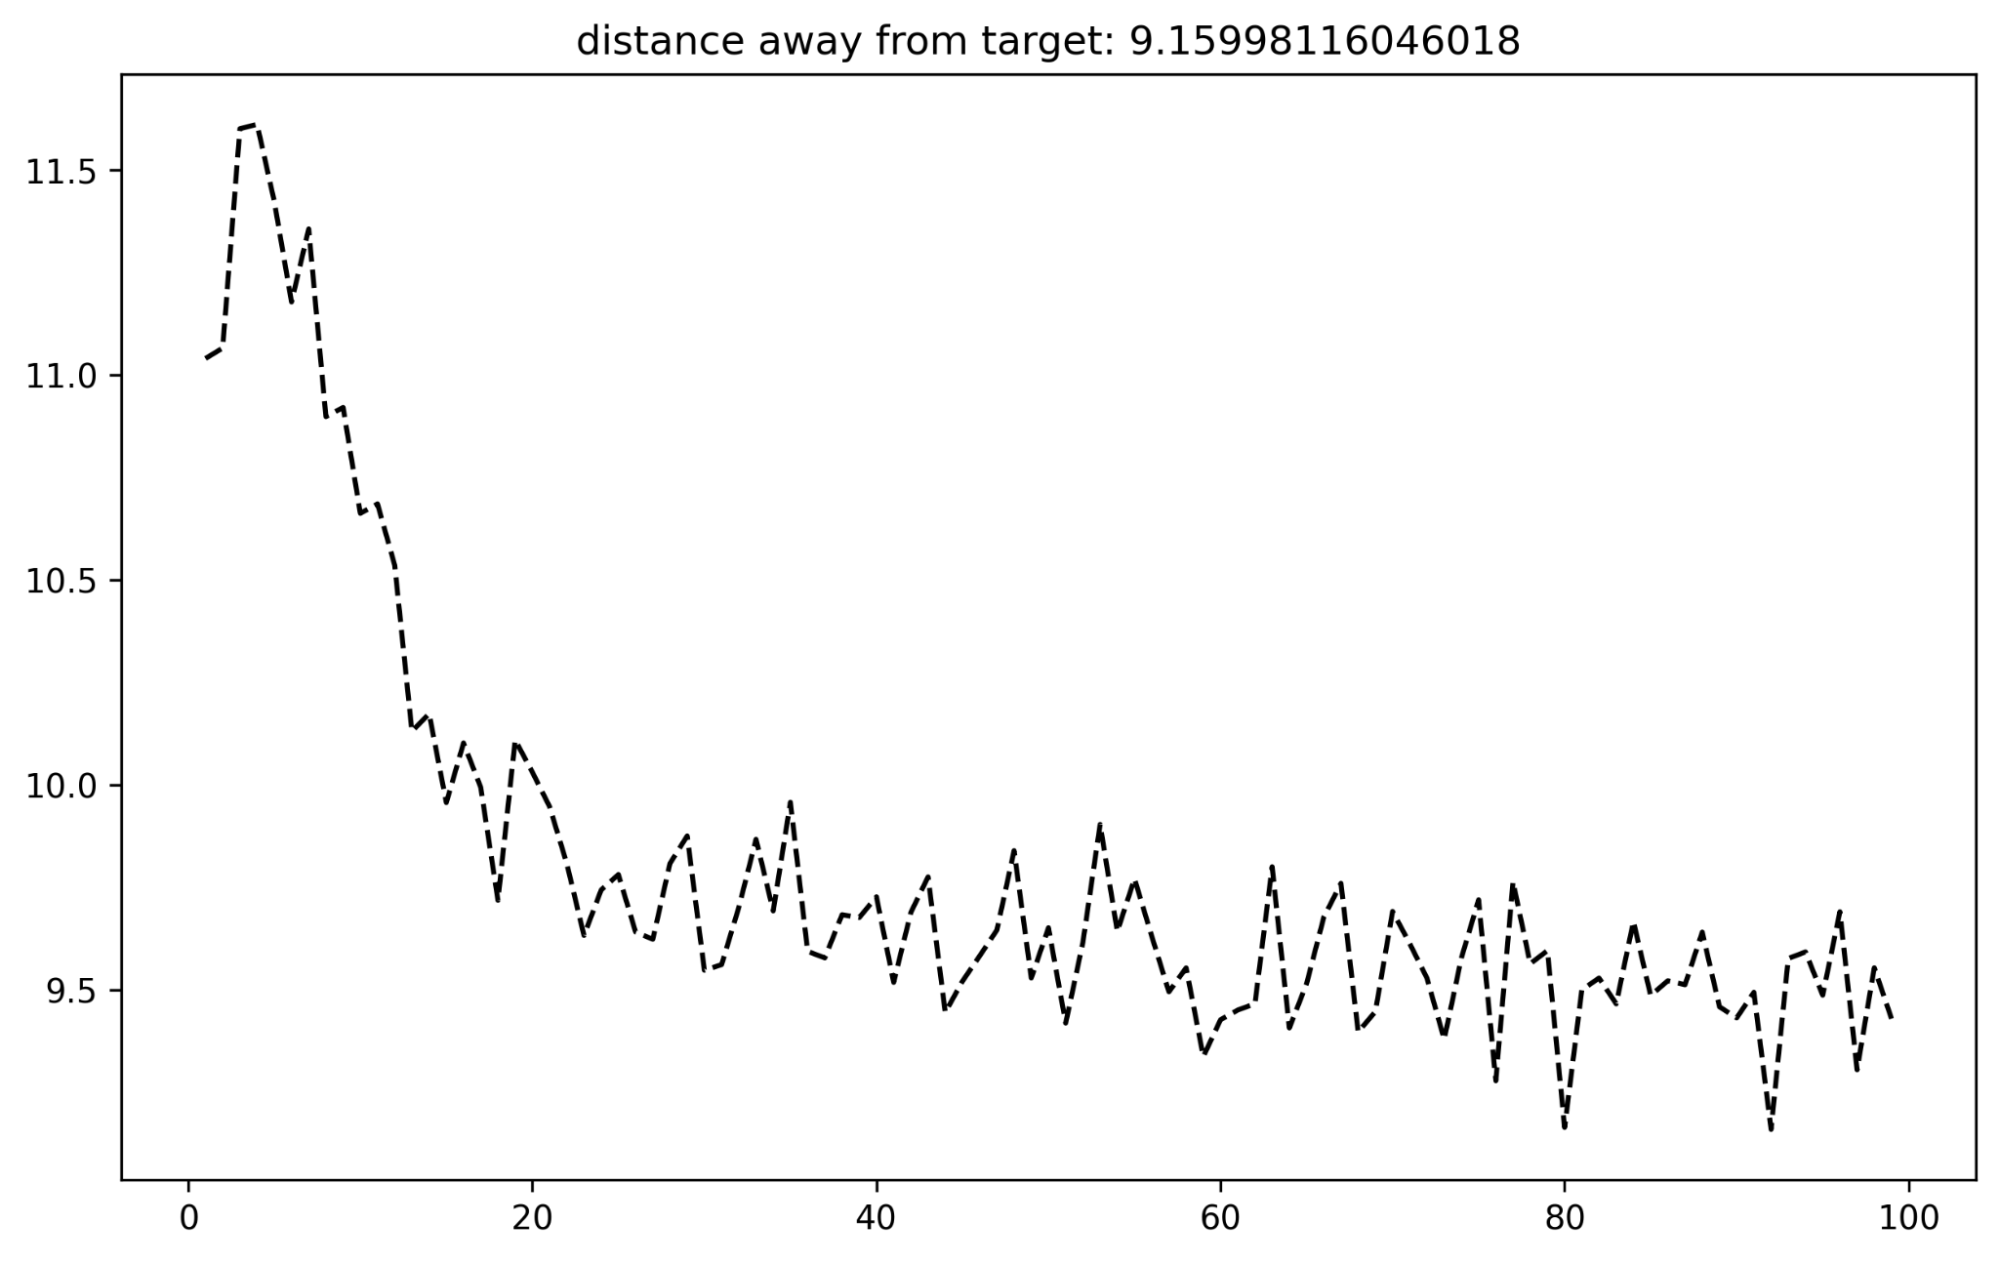
\includegraphics[width=\linewidth]{image7.png}
		\caption{RF Model AGT without BSSID filtering (1x1)}
		\label{fig:rf_agt_nofilter}
	\end{minipage}
\end{figure}

While the filtering method we applied was relatively simple, it had a surprisingly large impact on computational feasibility. Observing fig.~\ref{fig:rf_acc_filter} and~\ref{fig:rf_acc_nofilter}, by reducing the number of BSSID features from 1799 to 378, we were able to train models across a wide range of grid sizes (1×1 to 15×15) without overwhelming our hardware. In contrast, attempting to train on the full, unfiltered set quickly became impractical—our RTX 3080 Ti struggled even with the smallest grid size. Although we didn’t record exact runtimes, the difference in resource demands was stark. This raises questions about the actual utility of the full feature set and suggests that a more systematic study of feature selection or dimensionality reduction could be worthwhile in future works.

Fig.~\ref{fig:rf_agt_filter} and~\ref{fig:rf_agt_nofilter} suggest that filtering access points did not negatively impact the model's learning process. A comparison of training trajectories for the 1x1 grid experiment shows that the filtered model performed comparably to the unfiltered one, if not slightly better in terms of convergence. This suggests that reducing feature dimensionality not only accelerates training but may also make learning more stable.

From our observations we can conclude that AGT and grid size have an inverse relationship on all models. As grid-size increases the AGT decreases on every machine learning model. After creating models of 1x1 to 15x15 in increments of 2x2, we determined that 7x7m was the best model that balanced precision and accuracy for our test environment. This benefitted us as we were able to use these new measurements as empirical data upon which we could determine the best balance between grid-size and AGT. However; we must acknowledge that these results may not generalize to all environments due to different WiFi signal behaviour and building structures. Data filtration also aided in producing slightly better results with the BSSID filtered Model having an AGT of 15.16, and the non filtered Model having an AGT of 15.12. Filtering the dataset also had significant benefits to computational efficiency and efficacy for our project. For a single NVIDIA 3080 RTX Ti GPU, filtering our data was one of the best ways to create a model under this hardware limitation. This reduction in feature dimensionality not only accelerates training but may also contribute to more stable learning.





\section{Conclusion}
%\vspace{-9pt}
In conclusion, This paper extends prior work on classification-based IPS \cite{LRE1} by refining the implementation. Through our experiments across multiple grid sizes, we visualized the trade-offs between grid size and precision, showing that increasing grid size does not necessarily improve accuracy and may, in some cases, lead to worse performance. Our findings suggest that a 7×7m grid size offers the best balance between accuracy and precision, making it suitable for applications that require finer localization. However, we acknowledge that these results may not generalize to all environments due to variations in WiFi signal behavior and building structures.

Additionally, we implemented a simple filtering method to limit the number of WiFi BSSID features, preventing excessive model complexity while maintaining comparable performance to an unfiltered approach. This method significantly reduced training time and computational requirements, allowing us to complete model training across multiple grid sizes efficiently. Our results indicate that reducing feature dimensionality not only accelerates training but may also contribute to more stable learning. To better assess IPS performance, we introduced two new evaluation metrics—Average Grid from Target (AGT) and Average Distance from Target (ADT)—which provide a clearer understanding of prediction deviation. Ultimately, our study highlights key considerations in IPS design, particularly in grid size selection and feature filtering, and offers insights for improving indoor positioning accuracy in practical implementations.

To summarize, we believe that the usage of Average Grid from Target (AGT)
and Average Distance from Target (ADT) will be beneficial as it will help people with mapping clearer prediction deviation and allow them to better pick a grid-size that matches their intended need. We also believe that filtering the data for our models provides many benefits, specifically allowing the model to be more computationally efficient as well as allowing our model to get better results. A potential idea for future work is the implementation of On-Device Prediction for our Model. This would allow for less-latency and improved responsiveness. To increase the model’s accuracy it is also possible to take this work into a different direction by switching from treating the problem as discrete to continuous localisation model.

\nocite{bgp4, add2, add3, add4}
\bibliographystyle{splncs04}
\bibliography{references}

\end{document}
